\documentclass[11pt,a4paper]{article}

% ── Packages ──────────────────────────────────────────────
\usepackage[utf8]{inputenc}
\usepackage[T1]{fontenc}
\usepackage[margin=2.5cm]{geometry}
\usepackage{amsmath,amssymb,amsthm,mathtools,bm}
\usepackage{graphicx}
\usepackage{booktabs,array,tabularx,longtable,multirow}
\usepackage{enumitem}
\usepackage[table]{xcolor}
\usepackage[colorlinks=true,linkcolor=blue!60!black,citecolor=blue!60!black,urlcolor=blue!60!black]{hyperref}
\usepackage{natbib}
\usepackage{setspace}
\usepackage{fancyhdr}
\usepackage{titlesec}
\usepackage{float}
\usepackage{algorithm}
\usepackage{algpseudocode}
\usepackage{caption}
\usepackage{subcaption}
\usepackage{tikz}
\usetikzlibrary{arrows.meta,positioning}

% ── Page style ────────────────────────────────────────────
\pagestyle{fancy}
\fancyhf{}
\fancyhead[L]{}
\fancyhead[R]{\small\textsc{Spectral Augmentation of Panel Forecasts}}
\fancyfoot[C]{\small\thepage}
\renewcommand{\headrulewidth}{0.4pt}
\setlength{\headheight}{14pt}

% ── Colors ────────────────────────────────────────────────
\definecolor{accent}{RGB}{19,61,122}
\titleformat{\section}{\Large\bfseries\color{accent}}{\thesection}{1em}{}
\titleformat{\subsection}{\large\bfseries\color{accent!80}}{\thesubsection}{1em}{}
\titleformat{\subsubsection}{\normalsize\bfseries\color{accent!60}}{\thesubsubsection}{1em}{}

% ── Date ──────────────────────────────────────────────────
\newcommand{\paperdate}{April 2026}

% ── Math commands ─────────────────────────────────────────
\newcommand{\R}{\mathbb{R}}
\newcommand{\E}{\mathbb{E}}
\newcommand{\tr}{\mathrm{tr}}
\newcommand{\diag}{\mathrm{diag}}
\newcommand{\balpha}{\bm{\alpha}}
\newcommand{\clip}{\mathrm{clip}_{\mathrm{SR}}}

\theoremstyle{definition}
\newtheorem{definition}{Definition}[section]
\newtheorem{proposition}{Proposition}[section]

\setlength{\parskip}{0.4em}
\setlength{\parindent}{0em}

% ══════════════════════════════════════════════════════════
\begin{document}
\thispagestyle{empty}

% ── Title options (recommended: Option 1) ─────────────────
% Option 1: Spectral Augmentation of Panel Forecasts with Dynamic Mode Decomposition
% Option 2: Dynamic Mode Decomposition as Residual Spectral Augmentation for Cross-Sectional Investment Forecasts
% Option 3: Cross-Sectional Spectral Augmentation: Residual Dynamic Mode Decomposition for Investment Panels

\begin{center}
{\LARGE\bfseries\color{accent}
Spectral Augmentation of Panel Forecasts\\[6pt]
with Dynamic Mode Decomposition\par}
\vspace{1cm}
{\large
Oleg Roshka\\[6pt]
}
{\normalsize
Independent Researcher\\[6pt]
\paperdate
}
\end{center}

\vspace{0.5cm}

% ── Abstract ──────────────────────────────────────────────
\begin{abstract}
\noindent
We study cross-sectional investment intensity forecasting with spectral state-space methods. On a 93-actor multilayer panel, standalone spectral prediction using Dynamic Mode Decomposition (DMD) with a near-identity Kalman transition ($F = 0.99I$) achieves predictive $R^2 = 0.415$---far below per-actor AR(1) at $0.594$---because the uniform transition destroys mode-specific dynamics captured by the DMD basis. Replacing the transition with DMD's own reduced propagator $\tilde{A}$ partially repairs standalone performance to $R^2 = 0.486$, but the fundamental limitation remains: a single spectral basis cannot replicate actor-specific persistence. The recommended architecture is a two-stage pipeline: pooled AR(1) with fixed effects captures shared persistence (Stage~1, $R^2 = 0.591$), then a DMD-based Kalman filter on Stage~1 residuals captures cross-sectional rotational structure (Stage~2). The default augmented model uses per-mode diagonal dynamics ($F = \diag(\tilde{A}_r)$, $R^2 = 0.619$); a maximum-performance variant uses the full reduced operator ($F = \tilde{A}_r$, $R^2 = 0.630$, $\Delta R^2 = +0.036$ vs AR(1); CI $[+0.021, +0.054]$; permutation $p = 0.001$; 10/10 windows). The result generalises across all three panels: $+1.7$pp on a 146-firm CapEx/Revenue panel, $+2.5$pp on a 270-actor multi-ratio panel, and $+3.6$pp on the 93-actor multilayer panel, with confidence intervals excluding zero in all cases. An ablation ladder demonstrates that the gain requires learned per-mode dynamics on the residuals: projection-only models, naive Kalman ($F = 0.99I$), and residual dynamic factor models all fail. Crucially, a PCA basis with diagonal AR(1) on residual principal component scores ($R^2 = 0.617$) matches DMD/Kalman with diagonal $\tilde{A}_r$ ($R^2 = 0.615$), and Ridge regression ($R^2 = 0.632$) matches the full-$\tilde{A}_r$ variant ($R^2 = 0.629$). The gain is from the two-stage architectural principle with per-mode dynamics, not from DMD's Koopman structure specifically. Additional filter complexity provides zero gain. Separately, the spectral basis rotates at $25.8^\circ$/quarter with stable 8-mode dimensionality, and dual regularisation is essential for reconstruction quality.
\end{abstract}

\vspace{0.3cm}
\noindent\textbf{Keywords:} spectral augmentation, dynamic mode decomposition, Kalman filter, panel forecasting, investment gap estimation, state-space models, capital allocation

\noindent\textbf{JEL Classification:} C32, C38, C58, E22, G11

% ══════════════════════════════════════════════════════════
\section{Introduction}
\label{sec:intro}
% ══════════════════════════════════════════════════════════

Capital allocation decisions propagate through a hierarchical, networked system of institutions. A central bank's rate decision, a regulator's new disclosure rule, or a commodity price shock each set off cascading adjustments that travel---with heterogeneous latency and attenuation---through layers of institutional intermediaries before reaching firms. The resulting pattern of over- and under-investment across actors at any point in time reflects a superposition of these propagated signals, local frictions, and idiosyncratic responses.

Despite rich literatures on factor models \citep{fama1993common}, network effects in economics \citep{acemoglu2012network}, and spectral graph theory \citep{ortega2018graph}, to our knowledge no established framework jointly: (i)~decomposes how investment-relevant signals propagate through a heterogeneous actor hierarchy; (ii)~estimates actor-specific investment gaps as deviations from a structurally-informed benchmark; and (iii)~validates that the resulting gap estimates carry out-of-sample predictive content.

This paper addresses all three objectives. We develop a spectral state-space framework that represents the cross-sectional dynamics of investment intensity through a low-dimensional modal basis extracted via Dynamic Mode Decomposition (DMD), filtered through a Kalman model with dual regularisation at both the observation and transition levels. On raw panel levels, standalone spectral prediction is informative for structural decomposition but inferior to simple baselines for forecasting. After removing shared persistence via a pooled AR(1) with fixed effects, there remains forecastable cross-sectional residual structure that a \textbf{spectral augmentation} architecture can exploit.

\subsection{Preview of Results}

Throughout, we measure forecast performance by the out-of-sample coefficient of determination,
\begin{equation}
R^2 = 1 - \frac{\sum_{i,t}(y_{i,t} - \hat{y}_{i,t})^2}{\sum_{i,t}(y_{i,t} - \bar{y})^2},
\label{eq:r2}
\end{equation}
where $\hat{y}_{i,t}$ is the model's prediction and $\bar{y}$ is the grand mean of observed $y_{i,t}$ across all actor--quarter pairs in the test window. Using the test-period mean (rather than the training-period mean) as the denominator follows the convention for pooled panel $R^2$; all models share the same denominator, so comparative $\Delta R^2$ is unaffected. Per-window $R^2$ values are averaged across the 10 test windows.

Our main findings are:

\begin{enumerate}[nosep]
\item \textbf{Standalone diagnostic negative result.} On the 93-actor multilayer panel ($K = 8$), standalone DMD/Kalman with a near-identity transition ($F = 0.99I$) achieves predictive $R^2 = 0.415$, far below per-actor AR(1) at $0.594$. The uniform transition destroys mode-specific dynamics. Replacing $F$ with DMD's reduced propagator $\tilde{A}$ partially repairs performance to $R^2 = 0.486$, but the standalone spectral model remains $0.108$ below AR(1). The gain is mainly per-mode dynamics in the working SVD coordinates, not cross-mode propagation: $\diag(\tilde{A})$ captures 96\% of the full-$\tilde{A}$ gain (Section~\ref{sec:standalone}).

\item \textbf{Augmentation positive result.} The recommended architecture is a two-stage pipeline: pooled AR(1) with fixed effects (Stage~1, $R^2 = 0.591$), followed by a DMD-based Kalman filter on Stage~1 residuals (Stage~2). The augmented model achieves $R^2 = 0.630$ ($\Delta R^2 = +0.036$ vs AR(1); CI $[+0.021, +0.054]$; permutation $p = 0.001$; 10/10 windows). A parsimonious default using diagonal dynamics ($R^2 = 0.619$) is recommended for deployment (Section~\ref{sec:ablation_ladder}).

\item \textbf{Residual-stage ablation ladder.} The centrepiece evidence table demonstrates that the gain requires learned per-mode dynamics on the residuals. Projection-only models (PCA, DMD) actively destroy the pooled+FE result. Naive Kalman ($F = 0.99I$) and residual DFM also fail. A PCA basis with diagonal AR(1) on residual scores matches DMD/Kalman performance, and Ridge regression on lagged residuals also achieves comparable gains---the contribution is the two-stage architectural principle, not DMD's specific Koopman structure (Section~\ref{sec:ablation_ladder}).

\item \textbf{Cross-panel robustness.} The augmentation result generalises across all three benchmark panels: $+1.7$pp on a 146-firm CapEx/Revenue panel, $+2.5$pp on a 270-actor multi-ratio panel, and $+3.6$pp on the 93-actor multilayer panel. All confidence intervals exclude zero (Section~\ref{sec:cross_panel}).

\item \textbf{Structural spectral analysis.} The spectral basis on the 93-actor panel rotates at $25.8^\circ$ per quarter ($\sigma = 6.5^\circ$; null simulation: $75.3^\circ$) with stable 8-mode dimensionality across all 52 quarterly transitions. Dual regularisation---spherical observation covariance ($R = cI$) and regularised transition---is essential for spectral reconstruction quality. Rolling basis update provides the single largest modal $R^2$ gain ($+14.7$pp, CI $[+11.1, +17.2]$pp). These structural findings support the augmentation architecture (Sections~\ref{sec:structural_ladder}--\ref{sec:variance_decomp}).

\item \textbf{Economic content.} Both pooled and augmented investment gaps predict subsequent cross-sectional intensity revision ($\beta < 0$, $|t| > 10$), and both survive actor fixed effects with negative coefficients. The augmented model's gaps are less persistent and less predictable---consistent with signal absorption rather than economic-content degradation (Section~\ref{sec:economic}).

\item \textbf{Parsimony.} Additional filter complexity beyond the DMD-informed transition provides zero gain: spectralised noise covariances ($\Delta = 0.000$), state persistence across basis updates ($\Delta = -0.001$), and Kim-filter regime switching \citep{kim1994dynamic} are all tested and shown unnecessary (Section~\ref{sec:discussion}).
\end{enumerate}

\noindent Equally important is what \emph{does not} work: standalone spectral replacement of simple baselines, forecast-optimised reduced-rank regression (RRR) in the short-panel regime, emergence diagnostics, directed spectral operators, and return-based intensity all fail to improve or actively degrade performance.

\subsection{Scope and Evaluation Caveats}

Several features of our evaluation design should be kept in mind. First, the out-of-sample evaluation uses 10 non-overlapping annual test windows, each containing 4 quarterly observations; per-window $R^2$ estimates are therefore noisy. Second, hyperparameters ($K = 8$, EWM halflife $\tau = 12$Q, training window $T = 5$yr) are fixed across all panels; there is no inner cross-validation in the reported results. Third, only three panels are tested---all US-dominated---and gains are modest ($+1.7$ to $+3.6$pp). Fourth, the full-$\tilde{A}$ advantage over $\diag(\tilde{A})$ is statistically marginal ($p = 0.036$) and not uniform across panels. Fifth, the economic-validation regressions are predictive associations, not causal identification.

\subsection{Contribution}

Our contributions are diagnostic, methodological, and empirical:

\textbf{Diagnostic.} We identify the transition matrix as the bottleneck of standalone spectral state-space forecasting. The near-identity prior ($F = 0.99I$) that is essential for regularising the Kalman filter's state-space dynamics simultaneously destroys the mode-specific temporal structure captured by DMD. This diagnostic explains why spectral models that work well for structural decomposition (modal $R^2 = 0.696$) fail for forecasting (predictive $R^2 = 0.415$). The distinction is clean: reconstruction quality depends on the Kalman \emph{update} step (which corrects using the current observation), while forecasting depends on the \emph{predict} step (which relies entirely on $F$).

\textbf{Methodological.} We propose a two-stage spectral augmentation architecture that resolves the standalone limitation. Stage~1 captures shared persistence; Stage~2 captures cross-sectional rotational structure in the residuals. The key insight is that DMD-informed per-mode dynamics in the working reduced coordinates ($\diag(\tilde{A})$, 8 parameters) capture 96\% of the gain from the full reduced operator ($\tilde{A}$, 64 parameters)---the value-add is per-mode self-dynamics, not cross-mode propagation. We further show that in the short-panel ($N \gg T$) regime, DMD's implicit Koopman structural constraint dominates explicit forecast optimisation (RRR), a finding of independent methodological interest.

\textbf{Empirical.} We provide a systematic ablation of residual-stage models demonstrating that the forecasting gain requires learned per-mode dynamics on the residuals---projection-only, naive Kalman, and DFM models all fail---but is not specific to the DMD basis: PCA with diagonal AR(1) and Ridge regression achieve comparable gains. The augmentation result generalises across three panels of varying heterogeneity, with the largest gains on the most heterogeneous panel.

\subsection{Related Literature}

Our work connects to several strands. The investment gap concept relates to the capital allocation literature, including \citet{hsieh2009misallocation} and \citet{restuccia2017causes}; our gap is a forecasting-based deviation, not a structural measure. Our spectral approach builds on signal processing on graphs \citep{ortega2018graph,sandryhaila2013discrete} and Dynamic Mode Decomposition \citep{schmid2010dynamic,kutz2016dynamic}, adapted here for economic panel data. The state-space filtering component extends the dynamic factor model tradition \citep{stock2002forecasting,doz2012quasi} with the regularisation insights of \citet{ledoit2004well}. The two-stage residual modelling draws on the forecast combination literature \citep{bates1969combination,timmermann2006forecast}. The reduced-rank regression comparison relates to \citet{reinsel1998multivariate}. The economic validation relates to the capital allocation efficiency literature \citep{wurgler2000financial} and the predictability of corporate investment \citep{abel1983optimal}.


% ══════════════════════════════════════════════════════════
\section{Framework}
\label{sec:framework}
% ══════════════════════════════════════════════════════════

\subsection{Setup}

Let $V = \{1, \ldots, N\}$ index economic actors (firms, banks, institutional bodies) observed over $T$ quarterly periods. Each actor $i$ has an observed \emph{investment intensity} $y_{i,t} \in [0,1]$, constructed as a cross-sectional percentile rank of a type-specific investment measure (Section~\ref{sec:data}). The $N \times T$ panel $Y = [y_{i,t}]$ is the primary input.

\begin{definition}[Investment Gap]
\label{def:gap}
The investment gap for actor $i$ at time $t$ relative to a benchmark functional $\mathcal{B}$ is
\begin{equation}
\Delta_{i,t} = y_{i,t} - y^*_{i,t}, \qquad y^*_{i,t} = \mathcal{B}(Y_{1:t}, \theta),
\label{eq:gap}
\end{equation}
where $\Delta_{i,t} > 0$ indicates investment above the model-implied benchmark and $Y_{1:t}$ denotes the information set available at time $t$.
\end{definition}

The framework operates on a hierarchical actor universe spanning three layers (Figure~\ref{fig:hierarchy}). The benchmark $y^*_{i,t}$ is constructed through five processing steps---demeaning, basis extraction, Kalman filtering, online adaptation, and gap computation---described in Sections~\ref{sec:demean}--\ref{sec:gap_compute}. These building blocks are then assembled into the recommended two-stage forecasting pipeline (Section~\ref{sec:two_stage}, Figure~\ref{fig:pipeline}).

% ── Hierarchy figure ──────────────────────────────────────
\begin{figure}[H]
\centering
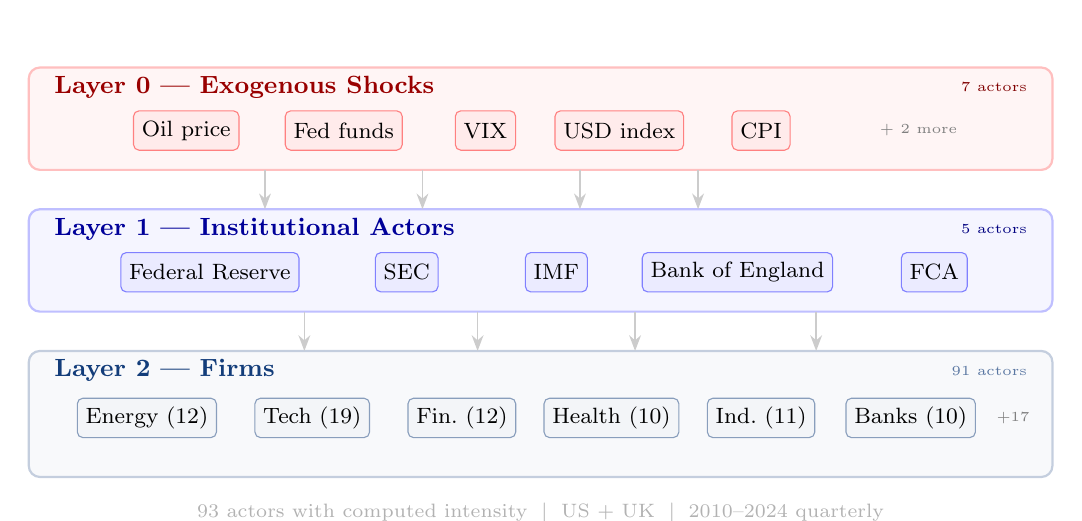
\begin{tikzpicture}[
  a0/.style={rectangle, draw=red!50, fill=red!8, rounded corners=2pt,
             font=\footnotesize, minimum height=0.5cm, inner sep=3pt},
  a1/.style={rectangle, draw=blue!50, fill=blue!8, rounded corners=2pt,
             font=\footnotesize, minimum height=0.5cm, inner sep=3pt},
  a2/.style={rectangle, draw=accent!50, fill=accent!5, rounded corners=2pt,
             font=\footnotesize, minimum height=0.5cm, inner sep=3pt},
  arr/.style={-{Stealth[length=2mm]}, color=gray!40, semithick},
  band/.style={rounded corners=4pt, thick}
]

% ── Layer 0 ───────────────────────────
\fill[red!4, band, draw=red!25] (-6.5, 3.05) rectangle (6.5, 4.35);
\node[font=\small\bfseries, text=red!60!black, anchor=west] at (-6.3, 4.1)
  {Layer 0 --- Exogenous Shocks};
\node[font=\tiny, text=red!50!black, anchor=east] at (6.3, 4.1) {7 actors};

\node[a0] at (-4.5, 3.55) {Oil price};
\node[a0] at (-2.5, 3.55) {Fed funds};
\node[a0] at (-0.7, 3.55) {VIX};
\node[a0] at (1.0, 3.55)  {USD index};
\node[a0] at (2.8, 3.55)  {CPI};
\node[font=\tiny, text=gray] at (4.8, 3.55) {+ 2 more};

% ── Layer 1 ───────────────────────────
\fill[blue!4, band, draw=blue!25] (-6.5, 1.25) rectangle (6.5, 2.55);
\node[font=\small\bfseries, text=blue!60!black, anchor=west] at (-6.3, 2.3)
  {Layer 1 --- Institutional Actors};
\node[font=\tiny, text=blue!50!black, anchor=east] at (6.3, 2.3) {5 actors};

\node[a1] at (-4.2, 1.75) {Federal Reserve};
\node[a1] at (-1.7, 1.75) {SEC};
\node[a1] at (0.2, 1.75)  {IMF};
\node[a1] at (2.5, 1.75)  {Bank of England};
\node[a1] at (5.0, 1.75)  {FCA};

% ── Layer 2 ───────────────────────────
\fill[accent!3, band, draw=accent!25] (-6.5, -0.85) rectangle (6.5, 0.75);
\node[font=\small\bfseries, text=accent, anchor=west] at (-6.3, 0.5)
  {Layer 2 --- Firms};
\node[font=\tiny, text=accent!70, anchor=east] at (6.3, 0.5) {91 actors};

\node[a2] at (-5.0, -0.1) {Energy (12)};
\node[a2] at (-2.9, -0.1) {Tech (19)};
\node[a2] at (-1.0, -0.1) {Fin.\ (12)};
\node[a2] at (0.9, -0.1)  {Health (10)};
\node[a2] at (2.8, -0.1)  {Ind.\ (11)};
\node[a2] at (4.7, -0.1)  {Banks (10)};
\node[font=\tiny, text=gray] at (6.0, -0.1) {+17};

% ── Arrows L0 → L1 ───────────────────
\foreach \x in {-3.5, -1.5, 0.5, 2.0} {
  \draw[arr] (\x, 3.05) -- (\x, 2.55);
}

% ── Arrows L1 → L2 ───────────────────
\foreach \x in {-3.0, -0.8, 1.2, 3.5} {
  \draw[arr] (\x, 1.25) -- (\x, 0.75);
}

% ── Bottom annotation ────────────────
\node[font=\scriptsize, text=gray!60, align=center] at (0, -1.3)
  {93 actors with computed intensity
   \;\textbar\; US + UK
   \;\textbar\; 2010--2024 quarterly};

\end{tikzpicture}
\caption{\textbf{Multilayer actor hierarchy.} The 103-actor universe spans three layers: exogenous shocks (Layer~0, FRED macro series), institutional intermediaries (Layer~1, central banks and regulators), and firms (Layer~2, US and UK equities and banks grouped by sector). Of these, 93 have computed investment intensity and enter the spectral analysis. The heterogeneous composition---mixing macro, institutional, and firm-level actors across sectors and geographies---creates the cross-sectional structure that the spectral augmentation architecture exploits.}
\label{fig:hierarchy}
\end{figure}

\subsection{Stage 1: Exponentially-Weighted Demeaning}
\label{sec:demean}

Investment intensity ranks exhibit strong cross-sectional persistence: an actor's mean rank is the single largest source of variance (51\% of total $R^2$ in the static-basis configuration; Section~\ref{sec:variance_decomp}). The state-space model $\tilde{y}_t = U\balpha_t + \varepsilon_t$ assumes zero-mean observations. We subtract an exponentially-weighted per-actor mean:
\begin{equation}
\hat{\mu}_i = \frac{\sum_{s=1}^{T} w_s \, y_{i,s}}{\sum_{s=1}^{T} w_s}, \qquad w_s = \exp\!\Bigl(-\frac{(T - s) \ln 2}{\tau}\Bigr),
\label{eq:ewm}
\end{equation}
with half-life $\tau = 12$ quarters. The demeaned observation is $\tilde{y}_{i,t} = y_{i,t} - \hat{\mu}_i$.

\subsection{Stage 2: Dynamic Mode Decomposition}
\label{sec:dmd}

Given the demeaned training panel $\tilde{Y} = [\tilde{y}_1, \ldots, \tilde{y}_T] \in \R^{N \times T}$, we extract a spectral basis that captures temporal cross-sectional dynamics.

\textbf{Why DMD over static operators.} Classical spectral approaches decompose a static operator (e.g., the cross-correlation matrix $C = \tilde{Y}\tilde{Y}^\top / T$). This captures contemporaneous co-movement but not lagged dynamics. DMD \citep{schmid2010dynamic} works with temporal snapshot pairs, capturing lagged cross-sectional dynamics invisible to contemporaneous decompositions.

\textbf{DMD algorithm.} Form snapshot matrices $X = [\tilde{y}_1, \ldots, \tilde{y}_{T-1}]$ and $X' = [\tilde{y}_2, \ldots, \tilde{y}_T]$. DMD seeks the best-fit linear operator $A$ such that $X' \approx AX$. Compute the truncated SVD $X = U_{\mathrm{svd}} \Sigma_r V_r^\top$, retaining $r$ singular values (we use $r = 15$, above which singular values are indistinguishable from noise). Form the reduced operator $\tilde{A} = U_{\mathrm{svd}}^\top X' V_r \Sigma_r^{-1} \in \R^{r \times r}$. We use the first $K = 8$ columns of $U_{\mathrm{svd}}$ as the modal basis $U \in \R^{N \times K}$ (projected DMD; this is the left-singular subspace of $X$, not the DMD eigenmodes). The full $r \times r$ operator $\tilde{A}$ is computed in the larger $r$-dimensional space; only the leading $K \times K$ block or its diagonal enters the transition matrix $F$.

\textbf{Why DMD over reduced-rank regression.} Reduced-rank regression (RRR; \citealt{reinsel1998multivariate}) directly minimises one-step prediction error by finding a rank-$K$ approximation to the OLS coefficient matrix. In the $N \gg T$ regime ($N = 93$, $T \approx 20$ quarters), the OLS coefficient is severely under-determined. DMD's dynamics-structured SVD decomposition acts as an implicit regulariser by constraining the solution to the Koopman operator subspace ($X' \approx AX$), which is a stronger structural prior than RRR's pure rank constraint. On the 93-actor panel, RRR loses to DMD at all $K$ values (Table~\ref{tab:standalone}).

\subsection{Stage 3: Kalman Filter with Spherical Observation Covariance}
\label{sec:kalman}

Given the modal basis $U \in \R^{N \times K}$, we model the latent modal dynamics as a linear Gaussian state-space system:
\begin{align}
\balpha_{t+1} &= F \balpha_t + \eta_t, \qquad \eta_t \sim \mathcal{N}(0, Q), \label{eq:state}\\
\tilde{y}_t &= U \balpha_t + \varepsilon_t, \qquad \varepsilon_t \sim \mathcal{N}(0, R). \label{eq:obs}
\end{align}

\textbf{Spherical observation regularisation.} The observation covariance $R \in \R^{N \times N}$ has $O(N^2)$ free parameters---estimated from $T = 20$ observations. We replace it with
\begin{equation}
R_{\mathrm{sph}} = \frac{\tr(\hat{R})}{N} \, I_N,
\label{eq:spherical}
\end{equation}
where $\hat{R}$ is the EM-estimated sample covariance. This reduces the parameter count from $O(N^2)$ to $O(1)$.

\textbf{Spectral radius clipping.} For any square matrix $M$, we define $\clip(M, c) = M \cdot \min(1,\; c / \rho(M))$, where $\rho(M)$ is the spectral radius. This rescales $M$ proportionally so that $\rho(\clip(M, c)) \leq c$, preserving the eigenvector structure while ensuring stability. For a diagonal matrix, this clips each entry individually: $[\clip(D, c)]_{kk} = D_{kk} \cdot \min(1, c/|D_{kk}|)$.

\textbf{Transition matrix options.} The transition $F \in \R^{K \times K}$ has $K^2$ free parameters. Three choices are relevant:
\begin{itemize}[nosep]
\item $F = 0.99 I_K$ (near-identity prior): a maximally regularised baseline that treats all modes identically. Section~\ref{sec:standalone} shows this destroys mode-specific dynamics and is the bottleneck of standalone forecasting.
\item $F = \clip(\diag(\tilde{A}), 0.99)$ (diagonal of the DMD reduced operator, clipped to spectral radius $\leq 0.99$): the recommended default, which preserves per-mode dynamics with $K$ parameters.
\item $F = \clip(\tilde{A}, 0.99)$ (full DMD reduced operator): the maximum-performance variant with $K^2$ parameters.
\end{itemize}

Together, spherical $R$ and the choice of transition define \emph{dual regularisation}: observation-level ($O(N^2) \to 1$) and transition-level ($K^2 \to K$ or $1$).

\subsection{Stage 4: Online State-Noise Adaptation}
\label{sec:online}

We augment the Kalman recursion with a recursive $Q$ update:
\begin{equation}
Q_{t+1} = (1 - \lambda)\, Q_t + \lambda\, (\balpha_{t|t} - F\balpha_{t-1|t-1})(\balpha_{t|t} - F\balpha_{t-1|t-1})^\top, \qquad \lambda = 0.3.
\label{eq:online_q}
\end{equation}
This tracks regime-dependent state volatility without explicit regime identification. Initial $Q_0 = 0.5\, I_K$.

\subsection{Stage 5: Gap Computation}
\label{sec:gap_compute}

The investment gap for actor $i$ at test time $t$ is:
\begin{equation}
\Delta_{i,t} = y_{i,t} - \underbrace{(\hat{\mu}_i + U\balpha_{t|t-1})}_{\displaystyle y^*_{i,t}},
\label{eq:gap_compute}
\end{equation}
where $\balpha_{t|t-1} = F\balpha_{t-1|t-1}$ is the Kalman-predicted modal state (using only information up to $t-1$).

\subsection{Two-Stage Spectral Augmentation Architecture}
\label{sec:two_stage}

The standalone pipeline (Stages~1--5 applied to raw panel levels) fails because a single spectral basis pools heterogeneous actors, losing actor-specific persistence that per-actor AR(1) captures. The recommended architecture resolves this by separating shared persistence from cross-sectional rotational structure.

\textbf{Stage~1: Pooled AR(1) with fixed effects.} Estimate a single persistence parameter $\hat{\rho}$ by within-transformation OLS on the training panel (pooling across all actors). The Stage~1 forecast is:
\begin{equation}
\hat{y}_{\mathrm{AR},i,t} = \hat{\mu}_i + \hat{\rho}\,(y_{i,t-1} - \hat{\mu}_i),
\label{eq:stage1}
\end{equation}
where $\hat{\mu}_i$ is the EWM per-actor mean (Eq.~\ref{eq:ewm}).

\textbf{Residual construction.} Training residuals are $r_{i,s} = y_{i,s} - \hat{y}_{\mathrm{AR},i,s}$ for $s$ in the training window.

\textbf{Stage~2: Residual DMD/Kalman.} Apply DMD to the EWM-demeaned training residuals, extracting a residual basis $U_r$ and reduced operator $\tilde{A}_r$ (subscript $r$ denotes ``residual-stage,'' distinguishing this from the standalone operator $\tilde{A}$). Run the Kalman filter (Eqs.~\ref{eq:state}--\ref{eq:obs}) on the residuals with:
\begin{equation}
F_r = \clip(\diag(\tilde{A}_r),\; 0.99) \quad \text{[default]}, \qquad\text{or}\quad F_r = \clip(\tilde{A}_r,\; 0.99) \quad \text{[max-performance]}.
\label{eq:Fr}
\end{equation}

\textbf{Combined forecast.} The final prediction is:
\begin{equation}
\hat{y}_{i,t} = \hat{y}_{\mathrm{AR},i,t} + [U_r \balpha_{t|t-1}^{(r)}]_i,
\label{eq:combined}
\end{equation}
where $\balpha_{t|t-1}^{(r)}$ is the residual-stage Kalman predicted state. The investment gap is $\Delta_{i,t} = y_{i,t} - \hat{y}_{i,t}$.

\textbf{Why this works.} Stage~1 captures shared persistence ($R^2 = 0.591$ on the 93-actor panel). Its residuals have near-zero persistence ($\rho \approx 0.04$) but retain cross-sectional structure: the residual spectral $R^2 = 0.095$. Stage~2's DMD basis captures the rotation patterns among actors after removing the persistence floor, and the Kalman filter with DMD-informed dynamics propagates these patterns forward for prediction.

\subsection{Summary: The Recommended Pipeline}

Algorithm~\ref{alg:pipeline} summarises the two-stage procedure.

\begin{algorithm}[H]
\caption{Two-Stage Spectral Augmentation (Recommended Pipeline)}
\label{alg:pipeline}
\begin{algorithmic}[1]
\Require Intensity panel $Y \in [0,1]^{N \times T}$, training window length, $K$ (typically 8), $\tau$ (typically 12Q), $\lambda = 0.3$
\Ensure Investment gaps $\Delta_{i,t}$ for test period
\State Compute EWM mean $\hat{\mu}_i$ from training period \Comment{Eq.~\eqref{eq:ewm}}
\State Estimate pooled AR(1) coefficient $\hat{\rho}$ by within-transformation OLS
\For{each test quarter $t$}
  \State \textbf{Stage~1 forecast:} $\hat{y}_{\mathrm{AR},i,t} = \hat{\mu}_i + \hat{\rho}(y_{i,t-1} - \hat{\mu}_i)$ \Comment{Eq.~\eqref{eq:stage1}}
  \State Compute training residuals $r_s = y_s - \hat{y}_{\mathrm{AR},s}$
  \State DMD on EWM-demeaned residuals $\to U_r, \tilde{A}_r$ \Comment{Section~\ref{sec:dmd}}
  \State Set $F_r = \clip(\diag(\tilde{A}_r), 0.99)$,\; $Q = 0.5 I_K$ \Comment{Eq.~\eqref{eq:Fr}}
  \State Estimate $R = \frac{\tr(\hat{R})}{N} I_N$ via single EM pass on training residuals \Comment{Eq.~\eqref{eq:spherical}}
  \State \textbf{Stage~2 Kalman predict:} $\balpha_{t|t-1}^{(r)} = F_r \balpha_{t-1|t-1}^{(r)}$
  \State \textbf{Combined forecast:} $\hat{y}_{i,t} = \hat{y}_{\mathrm{AR},i,t} + [U_r \balpha_{t|t-1}^{(r)}]_i$ \Comment{Eq.~\eqref{eq:combined}}
  \State \textbf{Predictive gap:} $\Delta_{i,t} = y_{i,t} - \hat{y}_{i,t}$ \Comment{Eq.~\eqref{eq:gap_compute}}
  \State Stage~2 Kalman update: $\balpha_{t|t}^{(r)}$ incorporating residual $\tilde{r}_t$
  \State Adapt: $Q \leftarrow (1-\lambda)Q + \lambda\,\mathrm{innov}\,\mathrm{innov}^\top$ \Comment{Eq.~\eqref{eq:online_q}}
  \State \textbf{Rolling update:} expand training; recompute $\hat{\mu}$, $\hat{\rho}$, $U_r$, $\tilde{A}_r$, $R$; reset $\balpha$, $P$, $Q$
\EndFor
\end{algorithmic}
\end{algorithm}

% ── Pipeline figure ───────────────────────────────────────
\begin{figure}[H]
\centering
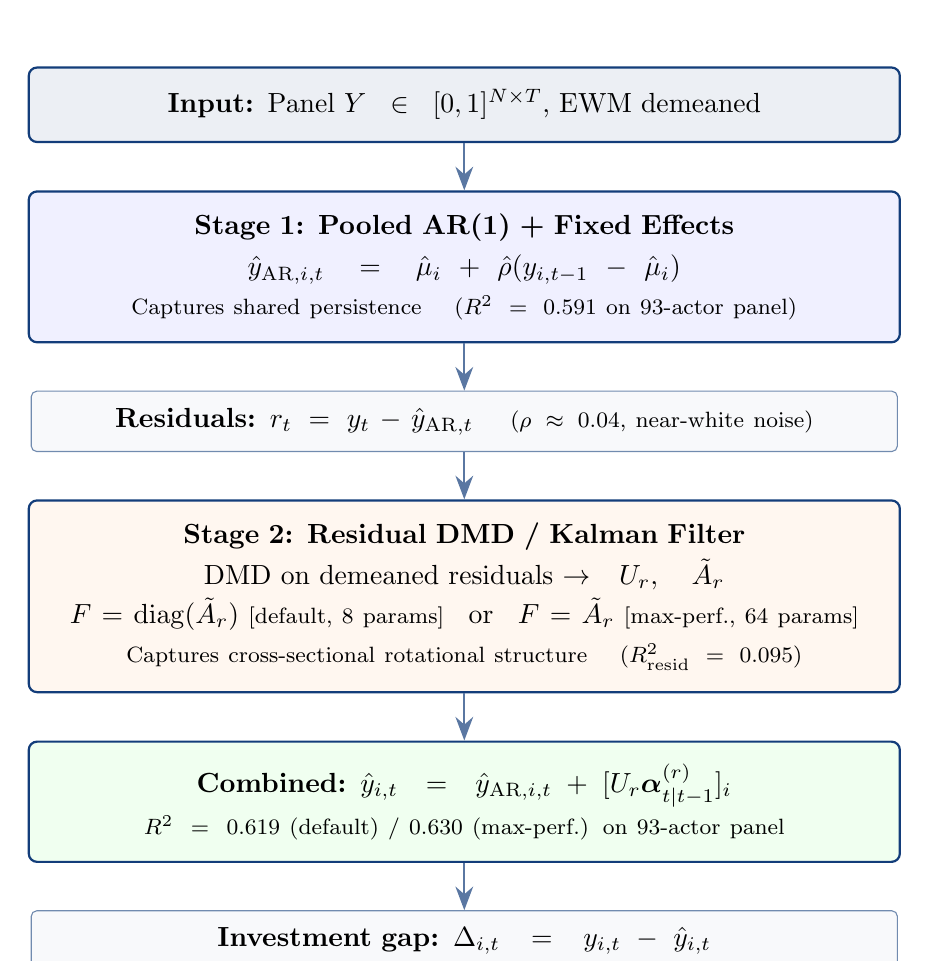
\begin{tikzpicture}[
  box/.style={rectangle, draw=accent, thick, rounded corners=3pt,
              minimum width=11cm, text width=10.5cm, align=center, inner sep=8pt},
  sbox/.style={rectangle, draw=accent!60, rounded corners=2pt,
              minimum width=11cm, text width=10.5cm, align=center, inner sep=6pt, fill=accent!3},
  arr/.style={-{Stealth[length=3mm]}, thick, color=accent!70},
  node distance=0.6cm
]
\node[box, fill=accent!8] (input)
  {\textbf{Input:} Panel $Y \in [0,1]^{N \times T}$, EWM demeaned};

\node[box, fill=blue!6, below=of input] (s1)
  {\textbf{Stage 1: Pooled AR(1) + Fixed Effects}\\[3pt]
   $\hat{y}_{\mathrm{AR},i,t} = \hat{\mu}_i + \hat{\rho}(y_{i,t-1} - \hat{\mu}_i)$\\[2pt]
   {\footnotesize Captures shared persistence \quad ($R^2 = 0.591$ on 93-actor panel)}};

\node[sbox, below=of s1] (resid)
  {\textbf{Residuals:} $r_t = y_t - \hat{y}_{\mathrm{AR},t}$ \quad
   {\footnotesize ($\rho \approx 0.04$, near-white noise)}};

\node[box, fill=orange!6, below=of resid] (s2)
  {\textbf{Stage 2: Residual DMD / Kalman Filter}\\[3pt]
   DMD on demeaned residuals $\to U_r,\; \tilde{A}_r$\\[2pt]
   $F = \diag(\tilde{A}_r)$ {\footnotesize [default, 8 params]} \;\;or\;\;
   $F = \tilde{A}_r$ {\footnotesize [max-perf., 64 params]}\\[2pt]
   {\footnotesize Captures cross-sectional rotational structure
   \quad ($R^2_{\mathrm{resid}} = 0.095$)}};

\node[box, fill=green!6, below=of s2] (comb)
  {\textbf{Combined:} $\hat{y}_{i,t} = \hat{y}_{\mathrm{AR},i,t}
   + [U_r \balpha_{t|t-1}^{(r)}]_i$\\[3pt]
   {\footnotesize $R^2 = 0.619$ (default) / $0.630$ (max-perf.) on 93-actor panel}};

\node[sbox, below=of comb] (gap)
  {\textbf{Investment gap:} $\Delta_{i,t} = y_{i,t} - \hat{y}_{i,t}$};

\draw[arr] (input) -- (s1);
\draw[arr] (s1) -- (resid);
\draw[arr] (resid) -- (s2);
\draw[arr] (s2) -- (comb);
\draw[arr] (comb) -- (gap);
\end{tikzpicture}
\caption{\textbf{Two-stage spectral augmentation architecture} (recommended pipeline). Stage~1 captures shared persistence via pooled AR(1) with fixed effects. Stage~2 applies DMD/Kalman to Stage~1 residuals, exploiting cross-sectional rotational structure that Stage~1 leaves behind. The default transition uses per-mode diagonal dynamics ($K$ parameters); the maximum-performance variant uses the full reduced operator ($K^2$ parameters). Both outperform per-actor AR(1) across all three panels (Table~\ref{tab:cross_panel}).}
\label{fig:pipeline}
\end{figure}


% ══════════════════════════════════════════════════════════
\section{Data}
\label{sec:data}
% ══════════════════════════════════════════════════════════

\subsection{Actor Universe}

Our sample comprises 103 actors across three hierarchical layers (Table~\ref{tab:actors}). Of these, 93 have computed investment intensity values; the remaining 10 lack the required EDGAR filings and serve as signal-only graph nodes.

\begin{table}[H]
\centering\small
\begin{tabular}{@{}lllrr@{}}
\toprule
Layer & Actor Type & Intensity Method & Total & With intensity \\
\midrule
0 (Exogenous) & Global shocks (Global) & FRED min-max & 7 & 7 \\
\multirow{3}{*}{1 (Institutional)} & Central banks (US, UK) & FRED min-max & 2 & 1 \\
 & Regulators (US, UK) & FRED min-max & 2 & 2 \\
 & International orgs (Global) & FRED min-max & 1 & 1 \\
\midrule
\multirow{4}{*}{2 (Firms)} & Large firms (US) & CapEx intensity & 56 & 49 \\
 & Large firms (UK) & Return intensity & 23 & 21 \\
 & Banks (US) & Asset growth (ranked) & 10 & 10 \\
 & Sector leaders (UK) & CapEx intensity & 2 & 2 \\
\midrule
& & \textbf{Total} & \textbf{103} & \textbf{93} \\
\bottomrule
\end{tabular}
\caption{Actor universe for the 93-actor multilayer panel. This panel is used for both structural spectral analysis and the primary forecasting evaluation. The 146-firm and 270-actor panels (Section~\ref{sec:cross_panel}) are constructed from EDGAR balance sheet data for cross-panel robustness.}
\label{tab:actors}
\end{table}

\subsection{Investment Intensity}

We construct several intensity measures, each mapped to a cross-sectional percentile rank in $[0,1]$ per quarter:

\begin{itemize}[nosep]
\item \textbf{CapEx/Assets intensity} (93-actor panel): ratio of capital expenditures to total assets, sourced from SEC EDGAR (XBRL), ranked cross-sectionally. This is the primary panel for ablation, structural analysis, and forecasting evaluation.
\item \textbf{CapEx/Revenue intensity} (146-firm panel): ratio of capital expenditures to revenues, ranked cross-sectionally. Used for cross-panel robustness.
\item \textbf{Multi-ratio} (270-actor panel): stacks CapEx/Revenue and Revenue/Assets columns for overlapping firms, creating virtual cross-sectional heterogeneity. Used for cross-panel robustness.
\item \textbf{Institutional intensity}: FRED-based macro indices, min-max normalised within actor type.
\end{itemize}

\begin{table}[H]
\centering\small
\begin{tabularx}{\textwidth}{@{}lll>{\raggedright\arraybackslash}X@{}}
\toprule
Source & Data & Frequency & Role in Pipeline \\
\midrule
SEC EDGAR & CapEx, Assets, Revenue (XBRL) & Quarterly & Intensity construction (primary) \\
Yahoo Finance & Equity total returns & Daily $\to$ quarterly & Intensity construction (UK alternative) \\
FRED & 28 macro series & Mixed $\to$ quarterly & Institutional intensity \\
\bottomrule
\end{tabularx}
\caption{Data sources. Only the intensity panel enters the recommended pipeline.}
\label{tab:sources}
\end{table}

\subsection{Evaluation Protocol}
\label{sec:eval}

We employ a \textbf{rolling out-of-sample} protocol with 10 non-overlapping annual test windows (2015--2024). For each test year, the model trains on the preceding 5 years (20 quarters) and predicts the 4 quarters of the test year. Within each test year, the basis and Stage~1 parameters are updated quarterly (rolling update, Algorithm~\ref{alg:pipeline}).

\textbf{Fixed hyperparameters.} $K = 8$ DMD modes, SVD truncation rank $r = 15$, EWM halflife $\tau = 12$ quarters, training window $T = 5$ years, $F_{\mathrm{reg}} = 0.99$ (spectral radius clip), $Q_0 = 0.5 I_K$, $\lambda = 0.3$. These are fixed across all panels and windows; there is no inner cross-validation.

\textbf{Inference.} We report mean $\Delta R^2$ across 10 windows, 95\% bootstrap CIs (10{,}000 window resamples), exact permutation $p$-values ($2^{10} = 1{,}024$ sign assignments), and window win counts.

\textbf{Notation summary.} Two $R^2$ types appear throughout:
\begin{table}[H]
\centering\small
\begin{tabular}{@{}lll@{}}
\toprule
Symbol & Definition & Usage \\
\midrule
Predictive $R^2$ & Uses $\balpha_{t|t-1}$ (info up to $t{-}1$ only) & All forecast comparisons \\
Modal $R^2$ & Uses $\balpha_{t|t}$ (incorporates current obs) & Structural analysis only \\
\bottomrule
\end{tabular}
\end{table}


% ══════════════════════════════════════════════════════════
\section{Empirical Results}
\label{sec:results}
% ══════════════════════════════════════════════════════════

Sections~\ref{sec:standalone}--\ref{sec:cross_panel} present the forecasting results using predictive $R^2$ on all panels. Sections~\ref{sec:structural_ladder}--\ref{sec:variance_decomp} present complementary structural spectral analysis using modal $R^2$ on the 93-actor panel.

\subsection{Standalone Transition Diagnostic}
\label{sec:standalone}

Table~\ref{tab:standalone} presents the standalone diagnostic: why does spectral forecasting on raw levels fail, and how much can transition repair recover?

\begin{table}[H]
\centering\small
\begin{tabular}{@{}llccc@{}}
\toprule
Model & Transition & $R^2$ & $\Delta$ vs AR(1) & $\Delta$ vs baseline \\
\midrule
Per-actor AR(1) & --- & 0.594 & --- & --- \\
Pooled + FE & --- & 0.591 & $-0.003$ & --- \\
\midrule
\multicolumn{5}{@{}l}{\emph{Standalone spectral model (93-actor panel, $K = 8$):}} \\
Spectral baseline & $F = 0.99I$ & 0.415 & $-0.179$ & --- \\
Spectral + $\diag(\tilde{A})$ & Per-mode dynamics & 0.483 & $-0.111$ & $+0.068$ \\
Spectral + full $\tilde{A}$ & Full reduced operator & 0.486 & $-0.107$ & $+0.071$ \\
\midrule
\multicolumn{5}{@{}l}{\emph{Forecast-optimised alternative:}} \\
RRR ($K = 2$) & Rank-constrained OLS & 0.391 & $-0.203$ & --- \\
RRR ($K = 4$) & Rank-constrained OLS & 0.368 & $-0.226$ & --- \\
RRR ($K = 8$) & Rank-constrained OLS & 0.347 & $-0.247$ & --- \\
\bottomrule
\end{tabular}
\caption{Standalone spectral model diagnostic arc (93-actor multilayer panel, 10 annual windows). Repairing the transition from $F = 0.99I$ to DMD's own $\tilde{A}$ closes 40\% of the gap to AR(1) but cannot overcome the fundamental limitation. The diagonal of $\tilde{A}$ captures 96\% of the full-$\tilde{A}$ gain ($0.483$ vs $0.486$), confirming that the signal is per-mode self-dynamics, not cross-mode coupling. Reduced-rank regression (RRR) loses at all $K$ values due to overfitting in the $N \gg T$ regime.}
\label{tab:standalone}
\end{table}

\textbf{The transition is the bottleneck.} The near-identity prior $F = 0.99I$ shrinks every mode's predicted state toward zero at the same rate, destroying the mode-specific temporal structure that DMD captures. Replacing $F$ with $\tilde{A}$ (the DMD reduced operator) recovers mode-specific dynamics: each mode's predicted state evolves according to its learned eigenvalue, including oscillatory components ($\theta \approx 44$--$91^\circ$). This closes 40\% of the gap ($+0.071$~pp), but standalone spectral model remains $0.107$~pp below AR(1).

\textbf{Per-mode dynamics, not propagation.} Testing the diagonal of $\tilde{A}$ in SVD coordinates shows that off-diagonal coupling contributes only $+0.003$ ($0.483$ vs $0.486$). The gain is from per-mode self-dynamics---each mode evolving at its own rate---not from cross-mode propagation. This finding limits the interpretive claims the paper can make about information transmission between actors.

\textbf{Shrinkage.} Sweeping the convex combination $F_\gamma = \gamma \tilde{A} + (1-\gamma) \cdot 0.99I$ yields optimal $\gamma = 0.75$ ($R^2 = 0.490$), confirming that the dynamics are real (big jump $\gamma = 0 \to 0.5$) but mild shrinkage helps ($+0.004$ over $\gamma = 1$).

\textbf{RRR fails in short panels.} Reduced-rank regression directly minimises one-step prediction error but produces a severely under-determined OLS coefficient ($N = 93$, $T \approx 20$). DMD's Koopman structural constraint ($X' \approx AX$) provides implicit regularisation that RRR's rank constraint cannot match. Subspace angles of $40$--$70^\circ$ confirm the two methods find genuinely different subspaces.

\subsection{Residual-Stage Ablation Ladder}
\label{sec:ablation_ladder}

Table~\ref{tab:ablation} is the centrepiece evidence table. It shows the effect of adding various second-stage models on top of the pooled+FE baseline.

\begin{table}[H]
\centering\small
\begin{tabular}{@{}lccc@{}}
\toprule
Residual-stage model & $R^2$ & $\Delta$ vs pooled & $\Delta$ vs AR(1) \\
\midrule
Pooled + FE only & 0.591 & --- & $-0.003$ \\
\midrule
\multicolumn{4}{@{}l}{\emph{Models that fail:}} \\
+ Residual AR(1) & 0.605 & $+0.014$ & $+0.011$ \\
+ Residual PCA projection & 0.404 & $-0.187$ & $-0.190$ \\
+ Residual PCA + VAR (DFM) & 0.577 & $-0.014$ & $-0.016$ \\
+ Residual DMD projection & 0.469 & $-0.122$ & $-0.125$ \\
+ Residual DMD/Kalman ($F = 0.99I$) & 0.471 & $-0.120$ & $-0.122$ \\
\midrule
\multicolumn{4}{@{}l}{\emph{Models that succeed:}} \\
+ Residual PCA + diag AR(1)\textsuperscript{$\dagger$} & 0.617 & $+0.026$ & $+0.023$ \\
+ Residual DMD/Kalman ($\diag(\tilde{A}_r)$) & 0.619 & $+0.028$ & $+0.025$ \\
+ Residual Ridge ($\alpha = 1.0$)\textsuperscript{$\dagger$} & \textbf{0.632} & $+0.041$ & $+0.038$ \\
+ Residual DMD/Kalman (full $\tilde{A}_r$) & \textbf{0.630} & $+0.039$ & $+0.036$ \\
\bottomrule
\end{tabular}
\caption{Residual-stage ablation ladder (93-actor panel, 10 windows). Projection-only models (PCA, DMD) \emph{destroy} the pooled+FE result. Naive Kalman ($F = 0.99I$) also hurts. The gain requires learned per-mode dynamics: among successful models, PCA + diagonal AR(1) matches DMD/Kalman diag ($0.617$ vs $0.619$), and Ridge regression matches DMD/Kalman full ($0.632$ vs $0.630$). The contribution is the two-stage architectural principle, not DMD's specific basis. \textsuperscript{$\dagger$}New baselines added in response to reviewer feedback.}
\label{tab:ablation}
\end{table}

The ablation ladder establishes four key points:

\emph{Projection alone hurts.} Both PCA and DMD projection-only models produce $R^2 < 0.47$---far below pooled+FE at $0.591$. The projection introduces reconstruction noise without a filtering step to suppress it.

\emph{Naive dynamics hurt.} Adding a Kalman filter with $F = 0.99I$ ($0.471$) or a PCA+VAR dynamic factor model ($0.577$) fails to improve over pooled+FE. The uniform-transition Kalman mis-specifies mode-specific dynamics; the DFM's full VAR overfits with $K^2 = 64$ parameters from $T \approx 20$ observations.

\emph{Per-mode dynamics are essential.} All four successful models---PCA + diagonal AR(1), DMD/Kalman diag, Ridge, and DMD/Kalman full---share the property of learning mode-specific or actor-specific persistence on the residuals.

\emph{The gain is not DMD-specific.} PCA + diagonal AR(1) on residual PC scores ($R^2 = 0.617$) matches DMD/Kalman with $\diag(\tilde{A}_r)$ ($0.619$; paired $t = -0.46$, $p > 0.6$). Ridge regression with $\alpha = 1.0$ ($R^2 = 0.632$) matches DMD/Kalman with full $\tilde{A}_r$ ($0.630$). The contribution is the two-stage architecture with per-mode dynamics, not the specific choice of spectral basis. DMD retains a practical advantage in interpretability (the modes have loadings that can be inspected) and in the structural spectral analysis, but the forecasting gain does not require it.

\subsection{Strong Baseline Comparison}
\label{sec:baselines}

Table~\ref{tab:baselines_strong} compares the augmented model against progressively stronger baselines on the 93-actor panel.

\begin{table}[H]
\centering\small
\begin{tabular}{@{}lcccccc@{}}
\toprule
Model & $R^2$ & $\Delta$ vs AR(1) & CI & Perm.\ $p$ & Wins \\
\midrule
Per-actor AR(1) & 0.594 & --- & --- & --- & --- \\
Pooled + FE & 0.591 & $-0.003$ & $[-0.015, +0.011]$ & 0.650 & --- \\
Layer-specific pooled + FE & 0.598 & $+0.004$ & $[-0.009, +0.021]$ & 0.349 & --- \\
DFM ($K = 8$) & 0.568 & $-0.026$ & $[-0.040, -0.011]$ & 0.994 & --- \\
\midrule
\textbf{Augmented (full $\tilde{A}_r$)}\textsuperscript{a} & \textbf{0.630} & $\mathbf{+0.036}$ & $[+0.021, +0.054]$ & \textbf{0.001} & \textbf{10/10} \\
\bottomrule
\end{tabular}
\caption{Strong baseline comparison (93-actor panel, 10 windows). Neither pooled+FE, layer-specific pooled+FE, nor DFM significantly outperform AR(1). Only the two-stage spectral augmentation model beats AR(1) with CIs excluding zero and all windows positive. Augmented vs layer-specific pooled+FE: $\Delta = +0.032$, CI $[+0.022, +0.042]$, 10/10 wins. \textsuperscript{a}Two-stage pipeline from Section~\ref{sec:two_stage} with full $\tilde{A}_r$ transition.}
\label{tab:baselines_strong}
\end{table}

\textbf{Default vs maximum-performance.} On the 93-actor panel, full $\tilde{A}_r$ ($R^2 = 0.630$) exceeds $\diag(\tilde{A}_r)$ ($R^2 = 0.619$) by $+0.011$ ($t(9) = 2.47$, $p = 0.036$, CI $[+0.003, +0.019]$, 7/10 wins). This is marginally significant. The $\diag(\tilde{A}_r)$ variant is the recommended default for parsimony (8 parameters vs 64) and for its superior performance on the 146-firm panel (Section~\ref{sec:cross_panel}).

\subsection{Cross-Panel Robustness}
\label{sec:cross_panel}

Table~\ref{tab:cross_panel} tests the augmentation architecture on all three benchmark panels.

\begin{table}[H]
\centering\small
\begin{tabular}{@{}lcccccccc@{}}
\toprule
Panel & $N$ & AR(1) & Pooled & Aug.\ diag & Aug.\ full & $\Delta_{\mathrm{full}}$ & CI & W \\
\midrule
146-firm CapEx/Rev & 146 & 0.728 & 0.745 & \textbf{0.749} & 0.745 & $+0.017$ & $[+0.009, +0.025]$ & 8/10 \\
270-actor multi-ratio & 270 & 0.728 & 0.738 & 0.745 & \textbf{0.753} & $+0.025$ & $[+0.019, +0.030]$ & 10/10 \\
93-actor multilayer & 93 & 0.594 & 0.591 & 0.619 & \textbf{0.630} & $+0.036$ & $[+0.021, +0.054]$ & 10/10 \\
\bottomrule
\end{tabular}
\caption{Cross-panel robustness. All three panels show augmentation gains with CIs excluding zero. Gains are largest on the most heterogeneous panel (93-actor, $+3.6$pp) and smallest on the most homogeneous (146-firm, $+1.7$pp). Bold indicates the better variant for each panel. On the 146-firm panel, the default $\diag(\tilde{A}_r)$ variant ($0.749$) \emph{outperforms} the full variant ($0.745$), reinforcing the parsimony recommendation.}
\label{tab:cross_panel}
\end{table}

The augmentation result is general: it holds across panels of different size ($N = 93$ to $270$), composition (multilayer vs single-ratio vs multi-ratio), and base persistence. The gains scale with panel heterogeneity---the 93-actor panel mixes FRED-based macro actors, central banks, regulators, and firms across US and UK, creating richer cross-sectional dynamics. The 146-firm panel (homogeneous US CapEx firms) shows the smallest gains. This pattern is consistent with DMD capturing cross-sectional rotational structure that is richer in more heterogeneous panels.

\textbf{Architecture recommendation.} The $\diag(\tilde{A}_r)$ variant is the recommended default: it matches or exceeds full $\tilde{A}_r$ on the 146-firm panel and is within $+0.011$ on the 93-actor panel. The full variant is a maximum-performance option that may be preferred when the marginal gain justifies the additional $K^2 - K$ parameters.

% ── Structural Spectral Analysis ──────────────────────────
\vspace{0.5em}
\noindent\textit{The following subsections present structural spectral analysis on the 93-actor panel using modal $R^2$ (spectral reconstruction quality). These findings are complementary to the forecasting results above: they characterise the spectral structure that the augmentation architecture exploits.}

\subsection{The Structural Performance Ladder}
\label{sec:structural_ladder}

Independent of the forecasting architecture (Section~\ref{sec:two_stage}), we ask: what pipeline components are needed to build a high-quality spectral \emph{reconstruction} of the cross-section? Figure~\ref{fig:structural_pipeline} shows the standalone reconstruction pipeline; Table~\ref{tab:ladder} decomposes its modal $R^2$ into seven additive steps; Figure~\ref{fig:ladder} visualises the cumulative gains. This structural analysis uses $\tau = 8$Q and $T = 5$yr (the configuration under which these components were originally developed); the forecasting pipeline uses $\tau = 12$Q (Section~\ref{sec:eval}).

% ── Structural reconstruction pipeline ────────────────────
\begin{figure}[H]
\centering
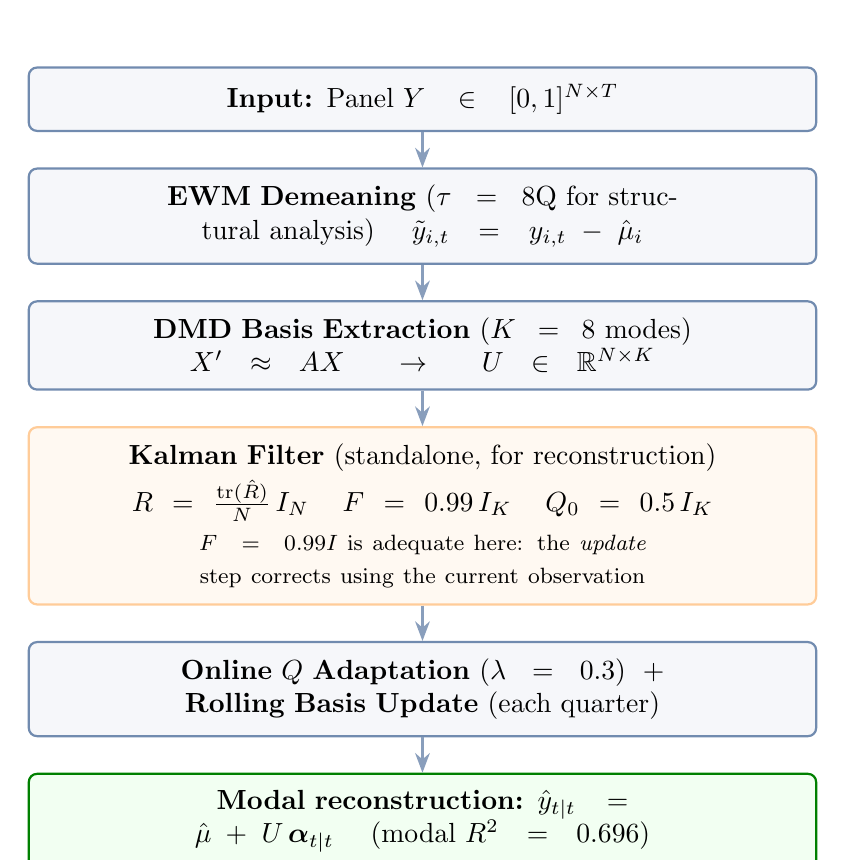
\begin{tikzpicture}[
  box/.style={rectangle, draw=accent!60, thick, rounded corners=3pt,
              minimum width=10cm, text width=9.5cm, align=center, inner sep=6pt,
              fill=accent!4},
  arr/.style={-{Stealth[length=2.5mm]}, thick, color=accent!50},
  node distance=0.45cm
]
\node[box] (input)
  {\textbf{Input:} Panel $Y \in [0,1]^{N \times T}$};

\node[box, below=of input] (ewm)
  {\textbf{EWM Demeaning} ($\tau = 8$Q for structural analysis)
   \quad $\tilde{y}_{i,t} = y_{i,t} - \hat{\mu}_i$};

\node[box, below=of ewm] (dmd)
  {\textbf{DMD Basis Extraction} ($K = 8$ modes)
   \quad $X' \approx AX \;\to\; U \in \R^{N \times K}$};

\node[box, fill=orange!5, draw=orange!40, below=of dmd] (kalman)
  {\textbf{Kalman Filter} (standalone, for reconstruction)\\[2pt]
   $R = \frac{\tr(\hat{R})}{N}\,I_N$ \;\;
   $F = 0.99\,I_K$ \;\;
   $Q_0 = 0.5\,I_K$\\[2pt]
   {\footnotesize $F = 0.99I$ is adequate here: the \emph{update} step
    corrects using the current observation}};

\node[box, below=of kalman] (online)
  {\textbf{Online $Q$ Adaptation} ($\lambda = 0.3$)
   \;+\; \textbf{Rolling Basis Update} (each quarter)};

\node[box, fill=green!5, draw=green!50!black, below=of online] (out)
  {\textbf{Modal reconstruction:}
   $\hat{y}_{t|t} = \hat{\mu} + U\,\balpha_{t|t}$
   \quad (modal $R^2 = 0.696$)};

\draw[arr] (input) -- (ewm);
\draw[arr] (ewm) -- (dmd);
\draw[arr] (dmd) -- (kalman);
\draw[arr] (kalman) -- (online);
\draw[arr] (online) -- (out);
\end{tikzpicture}
\caption{\textbf{Standalone reconstruction pipeline} (structural analysis only). This pipeline uses $F = 0.99I$ and the filtered state $\balpha_{t|t}$ to reconstruct the current cross-section (modal $R^2$). It is \emph{not} used for forecasting---the forecasting architecture (Figure~\ref{fig:pipeline}) replaces $F$ with DMD-informed dynamics and uses the predicted state $\balpha_{t|t-1}$. The structural ladder (Table~\ref{tab:ladder}, Figure~\ref{fig:ladder}) decomposes how each component of this pipeline contributes to reconstruction quality.}
\label{fig:structural_pipeline}
\end{figure}

\begin{figure}[H]
\centering
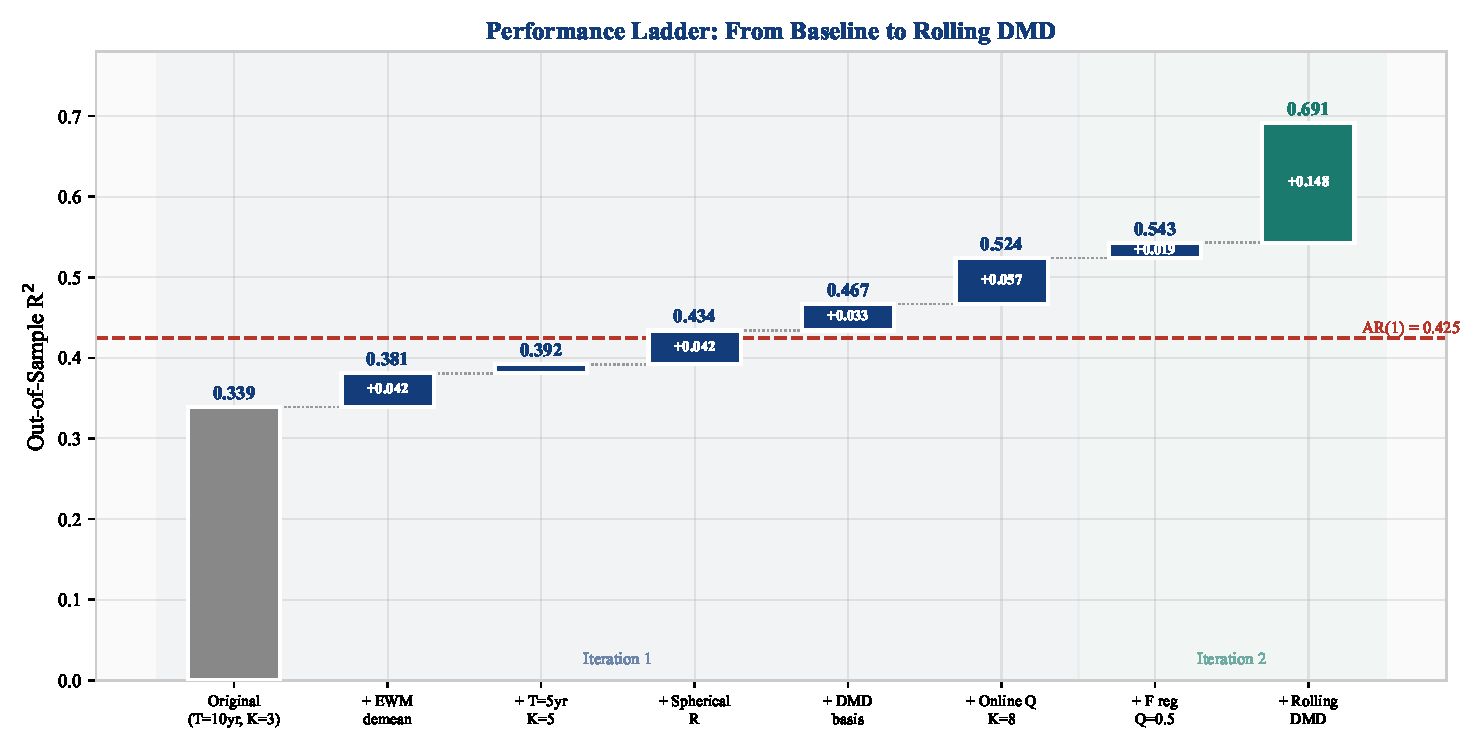
\includegraphics[width=0.95\textwidth]{img/fig2_ladder.pdf}
\caption{Structural performance ladder (93-actor panel, modal $R^2$): cumulative reconstruction quality across pipeline components shown in Figure~\ref{fig:structural_pipeline}. Steps~1--2 (not shown) cause Kalman divergence without spherical $R$. Rolling basis update provides the dominant gain ($+14.7$pp). See Table~\ref{tab:ladder} for per-step $\Delta R^2$ with bootstrap confidence intervals.}
\label{fig:ladder}
\end{figure}

\begin{table}[H]
\centering\footnotesize
\begin{tabularx}{\textwidth}{@{}lXcccc@{}}
\toprule
Step & Change & $R^2$ & $\Delta R^2$ & 95\% CI & Frac.\ + \\
\midrule
0 & Baseline ($T\!=\!10$yr, $K\!=\!3$, Schur, full demean) & 0.266 & --- & --- & --- \\
1 & + EWM demeaning ($\tau\!=\!8$Q) & $-0.89$ & $-1.16$ & \multicolumn{2}{c}{\emph{Kalman overfits}} \\
2 & + Shorter training ($T\!=\!5$yr) + higher $K\!=\!5$ & divergent & divergent & \multicolumn{2}{c}{\emph{without spherical $R$}} \\
3 & + Spherical $R$ in Kalman filter & 0.440 & +0.174 & --- & 100\% \\
\midrule
4 & + DMD basis (replacing Schur) & 0.472 & +0.033 & $[+0.006, +0.056]$ & 90\% \\
5 & + Online $Q$ adaptation + $K\!=\!8$ & 0.530 & +0.058 & $[+0.035, +0.092]$ & 100\% \\
6 & + Transition reg.\ $F\!=\!0.99I$, $Q_0\!=\!0.5I$ & 0.549 & +0.018 & $[+0.013, +0.024]$ & 100\% \\
7 & + Rolling basis update (recompute DMD each Q) & \textbf{0.696} & \textbf{+0.147} & $[+0.111, +0.172]$ & 100\% \\
\bottomrule
\end{tabularx}
\caption{Structural performance ladder with uncertainty (93-actor panel, modal $R^2$, 10 windows). Steps~1--2 demonstrate the overparameterisation failure; spherical $R$ (step~3) rescues the pipeline. Rolling basis update is the dominant effect. \textbf{Note:} This ladder uses $F = 0.99I$ (step~6), which is adequate for modal $R^2$ because the Kalman \emph{update} step corrects any transition mis-specification using the current observation. The transition choice matters for \emph{predictive} $R^2$ (Section~\ref{sec:standalone}), where only the predict step is available.}
\label{tab:ladder}
\end{table}

The distinction between modal and predictive $R^2$ explains why $F = 0.99I$ appears adequate in the structural ladder but catastrophic for forecasting. Modal $R^2$ measures $\hat{y}_{t|t} = \hat{\mu} + U\balpha_{t|t}$, where $\balpha_{t|t}$ incorporates the current observation through the Kalman update---correcting any mis-specification in $F$. Predictive $R^2$ measures $\hat{y}_{t|t-1} = \hat{\mu} + U\balpha_{t|t-1}$, where $\balpha_{t|t-1} = F\balpha_{t-1|t-1}$ depends entirely on $F$.

\subsection{Spectral Method Comparison}
\label{sec:spectral}

\begin{figure}[H]
\centering
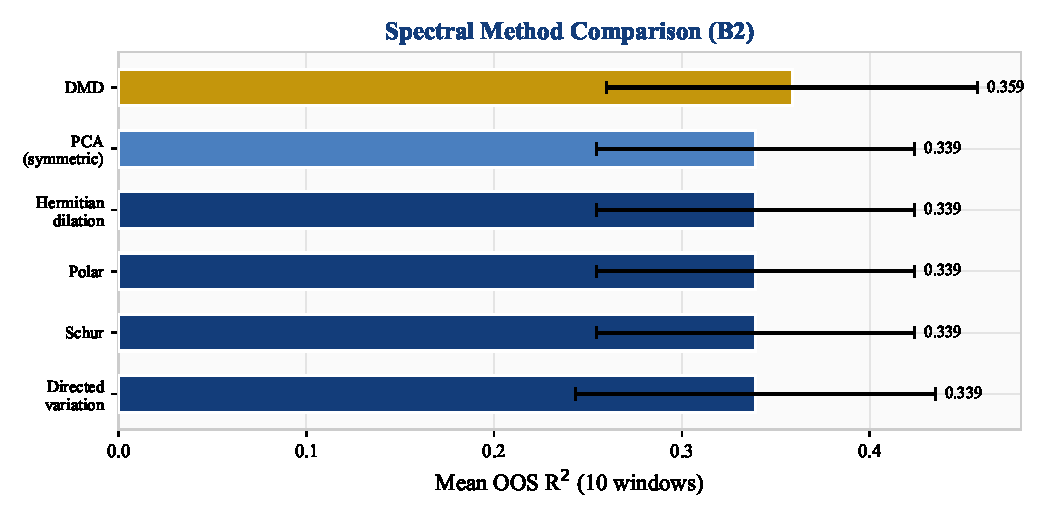
\includegraphics[width=0.7\textwidth]{img/fig5_spectral.pdf}
\caption{Spectral method comparison (93-actor panel, modal $R^2$, 10 windows). Five static-operator methods produce identical results because the operator is symmetric. DMD outperforms by $+2.0$pp because it captures lagged cross-sectional dynamics from temporal snapshot pairs.}
\label{fig:spectral}
\end{figure}

DMD ($R^2 = 0.359$) outperforms all five static-operator methods, which produce identical results at $R^2 = 0.339$. The identity is not a coincidence: the operator is built from the Pearson cross-correlation matrix, which is exactly symmetric. For any real symmetric matrix, the Schur, Polar, Hermitian, and PCA decompositions all reduce to the standard eigendecomposition. DMD sidesteps this by extracting modes from temporal snapshot pairs $X' \approx AX$, where the implicit operator captures lagged dynamics.

\subsection{The Regularisation Path}
\label{sec:reg_path}

\begin{figure}[H]
\centering
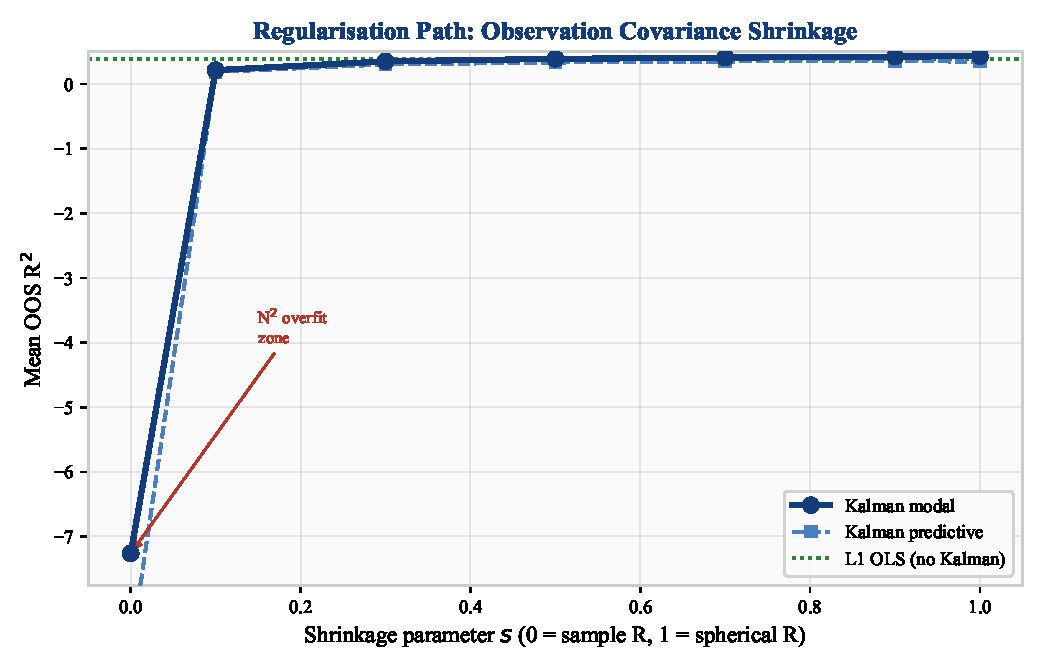
\includegraphics[width=0.75\textwidth]{img/fig6_regularisation.pdf}
\caption{Regularisation path (93-actor panel): $R^2$ as a function of shrinkage parameter $s$ where $R = (1-s)\hat{R} + s \cdot \frac{\tr(\hat{R})}{N}I$. At $s = 0$ (no shrinkage), modal $R^2 = -7.3$. Spherical $R$ ($s = 1.0$) is essential. The figure shows both modal $R^2$ (solid, incorporating current observation) and standalone predictive $R^2$ (dashed, one-step-ahead). The gap between the two curves illustrates the predict-step limitation identified in Section~\ref{sec:standalone}: even with correct observation regularisation, the standalone Kalman predict step underperforms because $F = 0.99I$ destroys mode-specific dynamics.}
\label{fig:reg}
\end{figure}

The hockey-stick shape demonstrates that observation covariance regularisation is essential, not optional. At $s = 0$, the Kalman filter diverges ($R^2 = -7.3$). Performance improves monotonically, reaching $R^2 = 0.43$ at $s = 1.0$ (spherical).

\subsection{Basis Rotation and Rolling Update}
\label{sec:rolling}

\begin{figure}[H]
\centering
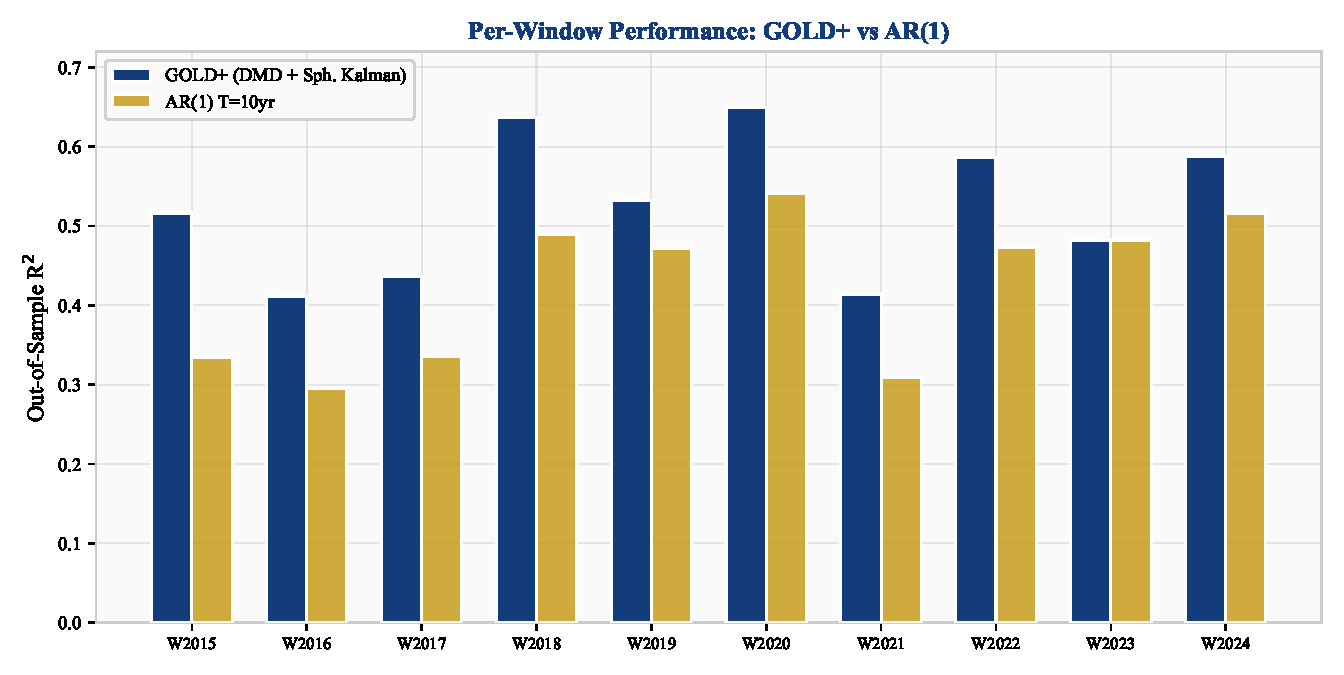
\includegraphics[width=\textwidth]{img/fig3_per_window.pdf}
\caption{Per-window modal $R^2$ (93-actor panel): rolling DMD vs static basis. Rolling wins all 10 windows, with the largest gains in periods where the cross-sectional structure shifts most from training.}
\label{fig:per_window}
\end{figure}

Tracking the DMD spectral basis across 52 rolling quarterly transitions (2010--2024) reveals gradual basis rotation (Figure~\ref{fig:rotation}). The mean principal subspace angle between successive quarterly bases is $25.8^\circ$ ($\sigma = 6.5^\circ$). High-rotation quarters ($>32^\circ$) tend to coincide with structural macroeconomic events: the European debt crisis (2012~Q3, $41^\circ$), the US--China tariff war (2018~Q2, $37^\circ$), and the Federal Reserve's tightening cycle (2022~Q3, $38^\circ$). COVID-19 (2020~Q2, $22^\circ$) did \emph{not} produce high rotation: the pandemic changed investment magnitudes but preserved the cross-sectional co-movement structure.

The \emph{dimensionality} of the spectral structure is stable: $K_{\mathrm{eff}} = 8$ modes in all 52 quarters, with zero mode births or deaths. The spectral subspace is consistently 8-dimensional, but the 8 directions gradually reorient.

\textbf{Null-simulation validation.} 500 panels from a fixed latent basis produce null rotation of $75.3^\circ$ ($\sigma = 1.5^\circ$)---far above the observed $25.8^\circ$. The observed rotation is consistent with reliably recoverable, low-dimensional structure that shifts gradually.

\begin{figure}[H]
\centering
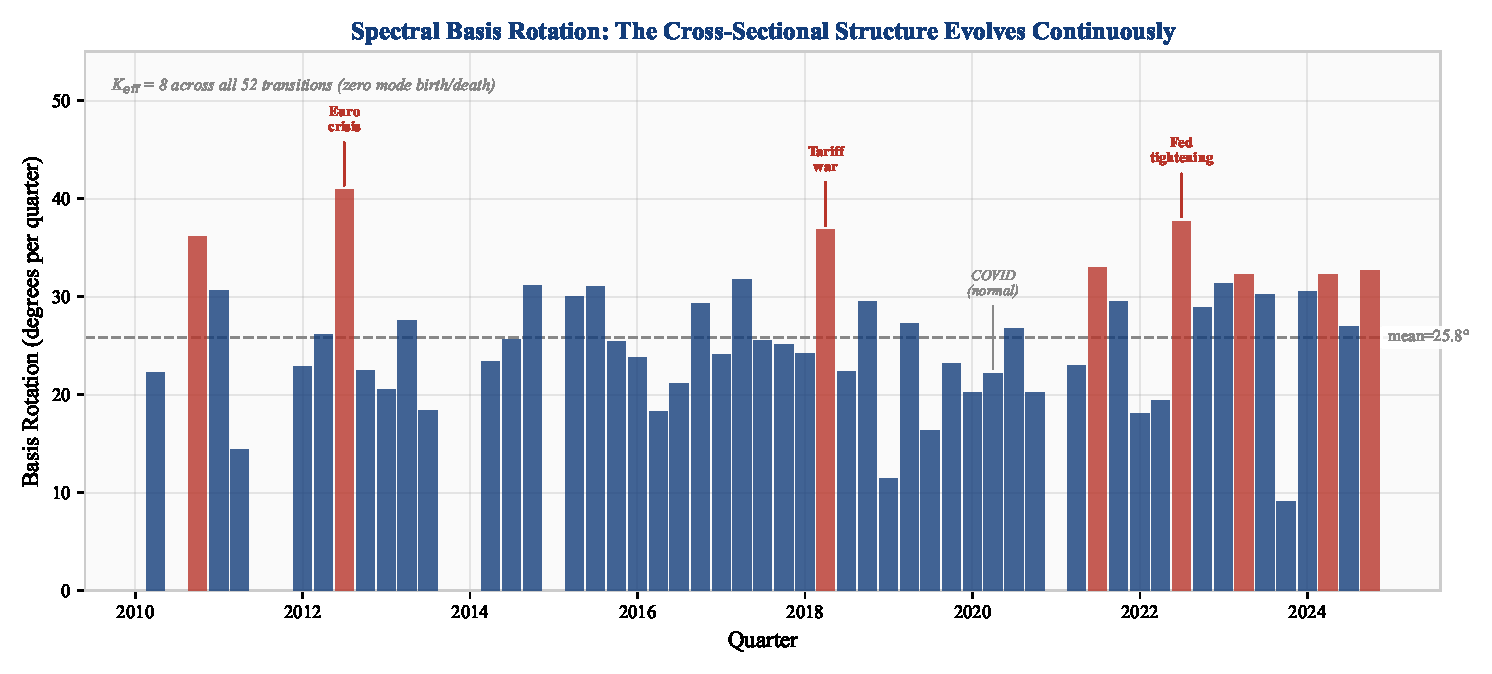
\includegraphics[width=\textwidth]{img/fig12_rotation.pdf}
\caption{Spectral basis rotation over time (93-actor panel). Each bar: principal subspace angle between successive quarterly DMD bases ($K = 8$). Red bars: high-rotation quarters ($>32^\circ$). Dashed line: mean ($25.8^\circ$). $K_{\mathrm{eff}} = 8$ in all quarters. Null simulation: $75.3^\circ$.}
\label{fig:rotation}
\end{figure}

Rolling basis update captures this rotation, yielding modal $R^2 = 0.696$---a $+14.7$pp improvement over the static-basis pipeline (CI $[+11.1, +17.2]$pp, 10/10 windows; Table~\ref{tab:rolling}).

\begin{table}[H]
\centering\small
\begin{tabular}{@{}lccc@{}}
\toprule
Configuration & Mean modal $R^2$ & Std & $\Delta$ (rolling $-$ static) \\
\midrule
Spectral (rolling basis) & \textbf{0.696} & 0.050 & $+0.147$ \\
Spectral (static basis) & 0.549 & 0.075 & --- \\
\bottomrule
\end{tabular}
\caption{Rolling vs static basis (93-actor panel, modal $R^2$, 10 windows).}
\label{tab:rolling}
\end{table}

\subsection{Variance Decomposition}
\label{sec:variance_decomp}

\begin{table}[H]
\centering\small
\begin{tabular}{@{}lccccc@{}}
\toprule
Source & \multicolumn{2}{c}{Static basis} & \multicolumn{2}{c}{Rolling basis} \\
\cmidrule(lr){2-3} \cmidrule(lr){4-5}
& $R^2$ & Share & $R^2$ & Share \\
\midrule
Per-actor EWM mean ($\hat{\mu}_i$) & 0.281 & 51\% & 0.281 & 40\% \\
Spectral dynamics ($U\balpha_{t|t}$) & 0.268 & 49\% & 0.415 & 60\% \\
\midrule
Total & 0.549 & 100\% & 0.696 & 100\% \\
\bottomrule
\end{tabular}
\caption{Variance decomposition (93-actor panel, modal $R^2$). Rolling basis recomputation shifts the balance from mean-dominated (51\%) to dynamics-dominated (60\%).}
\label{tab:variance}
\end{table}

\begin{figure}[H]
\centering
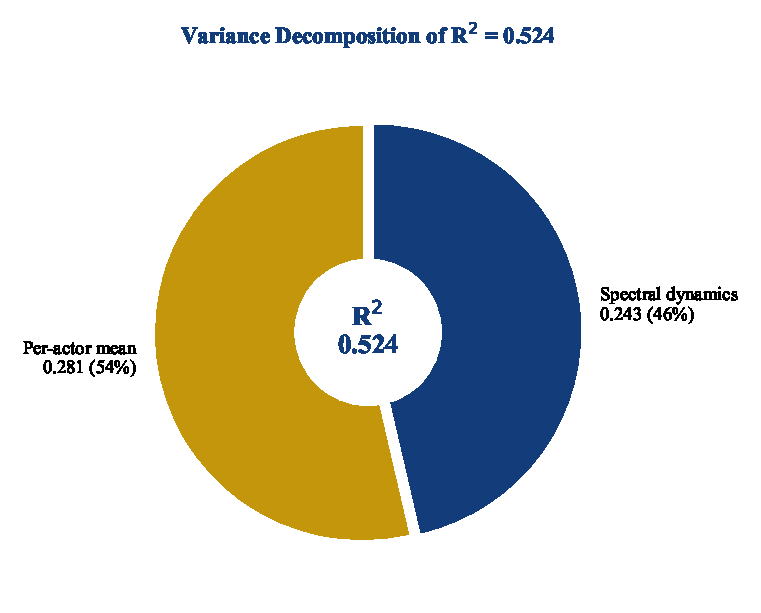
\includegraphics[width=0.85\textwidth]{img/fig11_variance.pdf}
\caption{Variance decomposition: frozen (left) vs rolling (right) basis. Rolling update nearly doubles the spectral dynamics contribution while the per-actor mean remains constant.}
\label{fig:variance}
\end{figure}

\subsection{Component Ablation}
\label{sec:comp_ablation}

A per-window heatmap of the reconstruction pipeline reveals a non-monotonic pattern: graph-factor OLS without Kalman filtering (modal $R^2 = 0.328$) \emph{outperforms} adding an unregularised Kalman filter ($0.291$) or adding regime switching ($0.293$). The Kalman filter hurts because the unregularised $R$ overfits. Spherical $R$ resolves this (SMIM static basis, $0.549$), and rolling basis update captures the structural evolution ($0.696$). The pattern is consistent across all 10 windows: unregularised Kalman is uniformly worse than no Kalman, and rolling basis is uniformly best.


% ══════════════════════════════════════════════════════════
\section{Economic Validation}
\label{sec:economic}
% ══════════════════════════════════════════════════════════

\subsection{What This Gap Is and Is Not}

The investment gap $\Delta_{i,t}$ is a \emph{model-implied} deviation: the difference between observed investment intensity and a benchmark prediction (Eq.~\ref{eq:gap_compute}). It is \emph{not} a welfare-theoretic misallocation measure in the sense of \citet{hsieh2009misallocation}. We use the term ``investment gap'' rather than ``misallocation'' and interpret positive results as evidence that the gap captures meaningful dynamics, not welfare losses.

\subsection{Gap Prediction Regressions}
\label{sec:gap_reg}

We estimate the panel regression:
\begin{equation}
\Delta y_{i,t \to t+4} = \beta_0 + \beta_1 \Delta_{i,t} + \beta_2 y_{i,t} + \epsilon_{i,t},
\label{eq:d2}
\end{equation}
where $\Delta y_{i,t \to t+4}$ is the next-4-quarter intensity change. Table~\ref{tab:econ_val} reports results for both pooled+FE gaps and augmented-model gaps, with and without actor fixed effects. The sample covers 93 actors across 40 quarters (2015~Q1 to 2024~Q4), yielding $3{,}348$ actor-quarter observations after excluding terminal quarters that lack 4 future quarters for the dependent variable.

\begin{table}[H]
\centering\small
\begin{tabular}{@{}llcccc@{}}
\toprule
Gap source & Specification & $\hat{\beta}_{\mathrm{gap}}$ & $t$-stat & $R^2$ \\
\midrule
Pooled + FE & No actor FE & $-0.589$ & $-27.8$ & 0.173 \\
Pooled + FE & Actor FE & $-0.630$ & $-10.3$ & 0.194 \\
\midrule
Augmented & No actor FE & $-0.530$ & $-23.1$ & 0.127 \\
Augmented & Actor FE & $-0.566$ & $-12.0$ & 0.142 \\
\bottomrule
\end{tabular}
\caption{Gap$\to$future revision regression (93-actor panel). Both pooled and augmented gaps predict subsequent intensity revision with strongly negative $\beta$ ($|t| > 10$). Crucially, \emph{both survive actor fixed effects} with negative coefficients: the gap-revision relationship holds within actors over time, not only cross-sectionally. Pooled gaps have slightly higher $|t|$ and $R^2$---see text for interpretation.}
\label{tab:econ_val}
\end{table}

\textbf{Both gap types survive actor FE.} Both pooled and augmented gaps maintain their negative revision coefficients under actor fixed effects. The within-actor effect ($\beta < 0$) means that when an individual actor deviates above its model-implied benchmark, it subsequently reverts---this holds both cross-sectionally and within actors over time.

\textbf{Pooled gaps are more predictive without FE.} Without actor fixed effects, pooled gaps have higher $|t|$ ($27.8$ vs $23.1$) and higher $R^2$ ($0.173$ vs $0.127$). Under actor FE, the comparison is mixed ($|t| = 10.3$ for pooled vs $12.0$ for augmented). This might seem paradoxical: the augmented model has higher forecast $R^2$, so why are its gaps \emph{less} predictable in the cross-sectional specification? The answer is signal absorption.

\subsection{Signal Absorption and Gap-Strength Decomposition}
\label{sec:signal_absorption}

\begin{table}[H]
\centering\small
\begin{tabular}{@{}lcccc@{}}
\toprule
Metric & Pooled gaps & Augmented gaps \\
\midrule
Gap cross-sectional $\sigma$ & 0.189 & 0.179 \\
Gap autocorrelation $\rho$ & 0.139 & 0.054 \\
Revision regression $|\beta|$ & 0.589 & 0.530 \\
Parent model OOS $R^2$ & 0.591 & 0.630 \\
\bottomrule
\end{tabular}
\caption{Gap-strength decomposition. Augmented gaps have lower variance, lower persistence, and lower revision predictability---consistent with the better model having absorbed systematic structure into the forecast, leaving residuals closer to white noise.}
\label{tab:gap_decomp}
\end{table}

The pattern is internally consistent: The augmented model's lower gap variance ($0.179$ vs $0.189$), lower persistence ($\rho = 0.054$ vs $0.139$), and lower revision $|\beta|$ ($0.530$ vs $0.589$) all indicate that the augmented model has moved systematic cross-sectional structure \emph{into} the forecast, leaving less predictable residuals. Stronger gap predictability can reflect a \emph{weaker} model leaving more exploitable structure in its residual. The contribution of the augmented architecture is predictive improvement ($R^2 = 0.630$ vs $0.591$), not stronger economic content of the gaps.


% ══════════════════════════════════════════════════════════
\section{Discussion}
\label{sec:discussion}
% ══════════════════════════════════════════════════════════

\subsection{Negative Results and Failed Extensions}

Several natural extensions of the spectral framework were tested and found unhelpful, establishing the boundaries of the approach.

Standalone DMD/Kalman on raw panel levels achieves $R^2 = 0.42$--$0.49$ depending on the transition---far below AR(1) at $0.594$. The spectral basis pools heterogeneous actors, losing actor-specific persistence. This is a fundamental limitation of the spectral representation, not a tuning problem. A forecast-optimised alternative, reduced-rank regression (RRR; \citealt{reinsel1998multivariate}), fares even worse: in the $N \gg T$ regime, the OLS coefficient is too under-determined for RRR's rank constraint to regularise effectively, whereas DMD's Koopman structural constraint provides stronger implicit regularisation.

On the residual stage, projection-only models (PCA and DMD without Kalman filtering) destroy the pooled+FE result ($R^2 = 0.40$--$0.47$ vs $0.591$), and a PCA+VAR dynamic factor model ($R^2 = 0.577$) is also worse than pooled+FE alone. The ablation ladder (Table~\ref{tab:ablation}) shows that the gain requires learned per-mode dynamics---but is not specific to DMD: PCA + diagonal AR(1) ($R^2 = 0.617$) and Ridge regression ($R^2 = 0.632$) achieve comparable results.

Three additional refinements to the Kalman filter were tested after establishing the augmentation result: (i)~spectralised noise covariances (diagonal $Q$, structured $R$) yield $\Delta = 0.000$; (ii)~projecting the Kalman state across basis updates yields $\Delta = -0.001$; (iii)~Kim-filter regime switching \citep{kim1994dynamic} is not warranted given (i)--(ii). The adaptive $Q$ (Eq.~\ref{eq:online_q}) already captures the needed dynamics; once the transition incorporates learned mode-specific information, further filter complexity adds nothing.

Emergence diagnostics (PID synergy, TDA complexity, Extended DMD), directed spectral operators (transfer entropy, Granger), event-level alignment, and return-based intensity were also tested and found to provide no improvement.

\subsection{Sources of Forecasting Gain}

The two-stage architecture succeeds by separating shared persistence (Stage~1) from cross-sectional rotational structure (Stage~2). The key mechanism is per-mode dynamics on the residuals: each component in the reduced space evolves at its own rate, capturing sector rotation and cross-sectional rebalancing patterns that shared-persistence models miss.

The gain is \emph{not} specific to DMD. PCA + diagonal AR(1) on residual PC scores matches DMD/Kalman diag ($R^2 = 0.617$ vs $0.619$; $p > 0.6$), and Ridge regression matches DMD/Kalman full ($0.632$ vs $0.630$). The contribution is the two-stage architectural principle---separate persistence from rotation, then learn per-mode dynamics on the residuals---not the choice of spectral basis. DMD retains practical value for interpretability (mode loadings reveal which actors co-move) and for the structural spectral analysis, but is interchangeable with PCA or Ridge for pure forecasting.

Nor is the gain evidence for directed propagation between actor layers. The diagonal of $\tilde{A}$ captures 96\% of the full-$\tilde{A}$ gain, and after removing shared persistence, residual modes are firm-dominated (macro loadings negligible). The forecastable structure reflects cross-sectional rotation among firms, not information transmission from macro actors to firms.

The augmentation gains scale with panel heterogeneity: $+1.7$pp on the homogeneous 146-firm panel, $+2.5$pp on the 270-actor multi-ratio panel, and $+3.6$pp on the heterogeneous 93-actor multilayer panel. Richer cross-sectional structure provides more exploitable rotational patterns. The structural spectral analysis explains \emph{why}: the cross-section lives in a stable 8-dimensional spectral subspace that rotates at $25.8^\circ$/quarter, and rolling basis recomputation is essential to track this evolution.

\subsection{Interpretive Boundaries}

Three interpretive boundaries deserve emphasis. First, the full reduced operator $\tilde{A}_r$ outperforms the diagonal variant on the 93-actor panel ($+0.011$, $p = 0.036$) but \emph{underperforms} it on the 146-firm panel ($0.745$ vs $0.749$). The diagonal variant is the more conservative and portable recommendation; the full variant is a maximum-performance option whose advantage is panel-dependent and statistically marginal.

Second, the augmented model's investment gaps are \emph{less} predictable than pooled gaps ($|\beta| = 0.530$ vs $0.589$; $\rho = 0.054$ vs $0.139$). This reflects signal absorption: the better model moves systematic structure into the forecast, leaving residuals closer to white noise. Weaker gap predictability is a sign of a better forecast, not a worse benchmark.

Third, the economic-validation regressions (Table~\ref{tab:econ_val}) establish that gaps predict subsequent intensity revision ($\beta < 0$, $|t| > 10$) both cross-sectionally and within actors. However, these are predictive associations, not causal identification. The gap measures deviation from a model-implied benchmark, not from a welfare-theoretic optimum.

\subsection{When the Kalman Filter Is and Is Not Needed}
\label{sec:simplification}

At low $K$ ($K = 2$) with quarterly basis refresh, the Kalman filter's contribution is marginal. The rolling update reprojects the modal state each quarter, and the subsequent predict step reduces to a scaled projection. The Kalman filter becomes essential at higher $K$ (the structural panel's $K = 8$ requires it for regularisation) and when the basis is not refreshed each quarter (online $Q$ adaptation tracks regime shifts between updates).

\subsection{Reading the Spectral Structure}

The structural analysis reveals that cross-sectional investment dynamics live in a stable 8-dimensional spectral subspace that rotates continuously.

\textbf{The 8 modes are investment co-movement themes.} Each DMD mode assigns a loading to every actor. Same-sign loadings indicate co-movement; opposite-sign loadings indicate substitution. These are empirically identified directions that cut across sector boundaries.

\textbf{$25.8^\circ$/quarter rotation means the themes drift.} Any model that is not re-estimated at least quarterly will track a structure that has shifted substantially.

\textbf{Rotation speed is diagnostic.} High-rotation quarters ($>32^\circ$) signal structural reorganisation of the investment co-movement map. This is distinct from volatility: VIX measures price movement magnitude; rotation measures how the co-movement structure rearranges.

\textbf{Stable dimensionality with shifting directions.} $K_{\mathrm{eff}} = 8$ is constant across all 52 transitions. No modes are born or die. The investment structure has a fixed number of degrees of freedom whose relative importance shifts gradually.

\subsection{Limitations}

\textbf{Panel scope.} Only three panels are tested, all US-dominated. Gains are modest ($+1.7$ to $+3.6$pp). The 270-actor multi-ratio panel stacks two ratios for approximately 135 overlapping firms, creating mechanical within-firm dependencies that the bootstrap does not explicitly account for; results on this panel should be interpreted with caution. Extending to international markets and sub-quarterly frequencies is open.

\textbf{Full $\tilde{A}_r$ advantage is marginal.} The $p = 0.036$ for diag vs full is not robust to multiple-testing correction and is not uniform across panels. The parsimony recommendation rests on this limitation.

\textbf{Remaining baselines.} PCA + diagonal AR(1) and Ridge regression are now included in the ablation ladder (Table~\ref{tab:ablation}). Elastic net and panel VAR with shrinkage priors (e.g., Minnesota-prior BVAR) are additional natural competitors not yet tested.

\textbf{Diagonal capture and estimation variance.} The finding that $\diag(\tilde{A})$ captures 96\% of the full-$\tilde{A}$ standalone gain could reflect either genuinely diagonal dynamics or superior estimation properties of the diagonal (8 parameters vs 64) in the $N \gg T$ regime. The fact that PCA + diagonal AR(1) matches DMD/Kalman diag (Table~\ref{tab:ablation}) is consistent with the latter interpretation: the gain comes from per-mode persistence estimation in any reasonable basis, not from DMD's specific Koopman structure.

\textbf{Economic validation.} The gap-revision regressions are predictive associations, not causal identification. The dependent variable $\Delta y_{i,t \to t+4}$ overlaps by 3 quarters for consecutive observations of the same actor, inducing MA(3) serial correlation. The reported $t$-statistics do not use Newey--West or Driscoll--Kraay standard errors and should be interpreted as indicative rather than exact. Additionally, the gap regressor is a generated variable (the residual from the forecasting model), which introduces pre-estimation uncertainty not reflected in the standard errors.

\textbf{Forecast metric.} We report only predictive $R^2$. Complementary metrics---RMSE, MAE, directional accuracy, and formal Diebold--Mariano tests \citep{diebold1995comparing} on loss differentials---would strengthen the forecast comparison.

\textbf{Inference.} Per-window $R^2$ estimates from 4 quarterly observations are noisy. With 10 windows whose 5-year training samples overlap by 80\% between adjacent years, the window-level statistics are not fully independent; the bootstrap CI and permutation test should be interpreted with this dependence in mind.

\textbf{Complex eigenvalues.} DMD of a real matrix can produce complex-conjugate eigenvalue pairs. In the implementation, all matrices are kept real: the basis $U$ consists of the real left-singular vectors of $X$, and $\tilde{A}$ is a real $r \times r$ matrix whose eigenvalues may be complex but whose matrix entries are real. The Kalman filter operates on real states throughout. The oscillatory components ($\theta \approx 44$--$91^\circ$) manifest as off-diagonal entries in the real $\tilde{A}$, not as explicit complex modes.


% ══════════════════════════════════════════════════════════
\section{Conclusion}
\label{sec:conclusion}
% ══════════════════════════════════════════════════════════

This paper presents three layers of findings on spectral state-space models for cross-sectional investment intensity forecasting.

\textbf{Diagnostic negative result.} Standalone spectral prediction using DMD with a near-identity Kalman transition ($F = 0.99I$) achieves $R^2 = 0.415$ on a 93-actor multilayer panel---far below per-actor AR(1) at $0.594$. The failure is implementation-specific: the uniform transition destroys mode-specific dynamics captured by the DMD basis. Replacing $F$ with DMD's reduced propagator partially repairs performance to $0.486$, but standalone spectral model cannot match simple baselines because a single spectral basis pools heterogeneous actors. In the $N \gg T$ regime, DMD's implicit Koopman constraint also dominates explicit forecast optimisation (reduced-rank regression), a finding of independent methodological interest.

\textbf{Methodological positive result.} The recommended architecture is a two-stage augmentation pipeline: pooled AR(1) with fixed effects captures shared persistence (Stage~1), then a second-stage model with learned per-mode dynamics on the residuals captures cross-sectional rotational structure (Stage~2). Using DMD/Kalman, the default model achieves $R^2 = 0.619$ ($\diag(\tilde{A}_r)$) and the maximum-performance variant $R^2 = 0.630$ (full $\tilde{A}_r$, $\Delta = +0.036$ vs AR(1); CI $[+0.021, +0.054]$; $p = 0.001$; 10/10 windows). The ablation ladder demonstrates that the gain requires learned per-mode dynamics---projection-only models, naive Kalman, and residual DFM all fail---but is not DMD-specific: PCA + diagonal AR(1) ($R^2 = 0.617$) and Ridge regression ($R^2 = 0.632$) achieve comparable results. The contribution is the two-stage architectural principle, not the choice of basis. Additional filter complexity provides zero gain.

\textbf{Empirical cross-panel robustness.} The augmentation result generalises across all three benchmark panels: $+1.7$pp on a 146-firm CapEx/Revenue panel, $+2.5$pp on a 270-actor multi-ratio panel, and $+3.6$pp on the 93-actor multilayer panel, with confidence intervals excluding zero throughout. Gains scale with panel heterogeneity. Both pooled and augmented investment gaps predict subsequent intensity revision ($\beta < 0$, $|t| > 10$), and both survive actor fixed effects---the gap-revision relationship holds within actors over time. The augmented model's gaps are less predictable, consistent with signal absorption: better forecasts leave less systematic structure in the residual.

Structural spectral findings complement these results. On the 93-actor panel ($K = 8$), the DMD basis rotates at $25.8^\circ$ per quarter ($\sigma = 6.5^\circ$; null: $75.3^\circ$) with stable dimensionality. Rolling basis recomputation provides the single largest structural gain ($+14.7$pp modal $R^2$). Dual regularisation---spherical observation covariance and regularised transition---is essential for reconstruction quality. The per-mode self-dynamics that drive the forecasting gain ($\diag(\tilde{A})$ captures 96\% of the full-$\tilde{A}$ effect) are consistent with sector rotation patterns in the spectral modes, not directed propagation between actor layers.

The broad methodological lesson is that \textbf{two-stage residual augmentation with learned per-mode dynamics} improves panel forecasts, regardless of whether the second-stage basis is DMD, PCA, or Ridge. DMD retains value for structural interpretability (the spectral analysis in Sections~\ref{sec:structural_ladder}--\ref{sec:variance_decomp} relies on it), but the forecasting contribution is the architectural principle: separate persistence from rotation, then learn component-specific dynamics on the residuals.

\vspace{0.8cm}
\noindent\textbf{Acknowledgements.} The author used Claude (Anthropic) for coding assistance, exploratory analysis support, and editorial feedback. All scientific decisions, interpretations, and claims remain the sole responsibility of the author.

\vspace{0.8cm}
\noindent\textbf{Disclaimer.} This paper presents a research framework for academic investigation of investment dynamics. It is not investment advice. The models, gap estimates, and statistical findings described herein have not been validated for live trading or portfolio construction. Past out-of-sample performance on historical data does not guarantee future results.

\vspace{0.5cm}

% ══════════════════════════════════════════════════════════
\begin{thebibliography}{99}

\bibitem[Bates and Granger(1969)]{bates1969combination}
Bates, J.~M. and Granger, C.~W.~J. (1969).
\newblock The combination of forecasts.
\newblock \emph{Journal of the Operational Research Society}, 20(4):451--468.

\bibitem[Abel and Blanchard(1983)]{abel1983optimal}
Abel, A.~B. and Blanchard, O.~J. (1983).
\newblock An intertemporal model of saving and investment.
\newblock \emph{Econometrica}, 51(3):675--692.

\bibitem[Acemoglu et~al.(2012)]{acemoglu2012network}
Acemoglu, D., Carvalho, V.~M., Ozdaglar, A., and Tahbaz-Salehi, A. (2012).
\newblock The network origins of aggregate fluctuations.
\newblock \emph{Econometrica}, 80(5):1977--2016.

\bibitem[Diebold and Mariano(1995)]{diebold1995comparing}
Diebold, F.~X. and Mariano, R.~S. (1995).
\newblock Comparing predictive accuracy.
\newblock \emph{Journal of Business \& Economic Statistics}, 13(3):253--263.

\bibitem[Doz et~al.(2012)]{doz2012quasi}
Doz, C., Giannone, D., and Reichlin, L. (2012).
\newblock A quasi-maximum likelihood approach for large, approximate dynamic factor models.
\newblock \emph{The Review of Economics and Statistics}, 94(4):1014--1024.

\bibitem[Fama and French(1993)]{fama1993common}
Fama, E.~F. and French, K.~R. (1993).
\newblock Common risk factors in the returns on stocks and bonds.
\newblock \emph{Journal of Financial Economics}, 33(1):3--56.

\bibitem[Kim(1994)]{kim1994dynamic}
Kim, C.-J. (1994).
\newblock Dynamic linear models with {M}arkov-switching.
\newblock \emph{Journal of Econometrics}, 60(1--2):1--22.

\bibitem[Hsieh and Klenow(2009)]{hsieh2009misallocation}
Hsieh, C.-T. and Klenow, P.~J. (2009).
\newblock Misallocation and manufacturing TFP in China and India.
\newblock \emph{The Quarterly Journal of Economics}, 124(4):1403--1448.

\bibitem[Kutz et~al.(2016)]{kutz2016dynamic}
Kutz, J.~N., Brunton, S.~L., Brunton, B.~W., and Proctor, J.~L. (2016).
\newblock \emph{Dynamic Mode Decomposition: Data-Driven Modeling of Complex Systems}.
\newblock SIAM.

\bibitem[Ledoit and Wolf(2004)]{ledoit2004well}
Ledoit, O. and Wolf, M. (2004).
\newblock A well-conditioned estimator for large-dimensional covariance matrices.
\newblock \emph{Journal of Multivariate Analysis}, 88(2):365--411.

\bibitem[Ortega et~al.(2018)]{ortega2018graph}
Ortega, A., Frossard, P., Kova{\v{c}}evi{\'c}, J., Moura, J.~M., and Vandergheynst, P. (2018).
\newblock Graph signal processing: Overview, challenges, and applications.
\newblock \emph{Proceedings of the IEEE}, 106(5):808--828.

\bibitem[Reinsel and Velu(1998)]{reinsel1998multivariate}
Reinsel, G.~C. and Velu, R.~P. (1998).
\newblock \emph{Multivariate Reduced-Rank Regression: Theory and Applications}.
\newblock Springer.

\bibitem[Restuccia and Rogerson(2017)]{restuccia2017causes}
Restuccia, D. and Rogerson, R. (2017).
\newblock The causes and costs of misallocation.
\newblock \emph{Journal of Economic Perspectives}, 31(3):151--174.

\bibitem[Sandryhaila and Moura(2013)]{sandryhaila2013discrete}
Sandryhaila, A. and Moura, J.~M. (2013).
\newblock Discrete signal processing on graphs.
\newblock \emph{IEEE Transactions on Signal Processing}, 61(7):1644--1656.

\bibitem[Schmid(2010)]{schmid2010dynamic}
Schmid, P.~J. (2010).
\newblock Dynamic mode decomposition of numerical and experimental data.
\newblock \emph{Journal of Fluid Mechanics}, 656:5--28.

\bibitem[Stock and Watson(2002)]{stock2002forecasting}
Stock, J.~H. and Watson, M.~W. (2002).
\newblock Forecasting using principal components from a large number of predictors.
\newblock \emph{Journal of the American Statistical Association}, 97(460):1167--1179.

\bibitem[Timmermann(2006)]{timmermann2006forecast}
Timmermann, A. (2006).
\newblock Forecast combinations.
\newblock In Elliott, G., Granger, C.~W.~J., and Timmermann, A., editors,
  \emph{Handbook of Economic Forecasting}, volume~1, pages 135--196. Elsevier.

\bibitem[Wurgler(2000)]{wurgler2000financial}
Wurgler, J. (2000).
\newblock Financial markets and the allocation of capital.
\newblock \emph{Journal of Financial Economics}, 58(1--2):187--214.

\end{thebibliography}

\end{document}
